\documentclass[12pt]{report}

\usepackage{amssymb, fullpage, amsmath,mathtools}
\usepackage{graphicx}

\newtheorem{problem}{Problem}

\newenvironment{solution}[1][\it{Solution}]{\textbf{#1. } }{$\square$}

\graphicspath{ {./} }

\allowdisplaybreaks

\pagestyle{empty}

\def\Z{{\mathbb Z}}
\def\Q{{\mathbb Q}}
\def\C{{\mathbb C}}
\def\R{{\mathbb R}}
\def\N{{\mathbb N}}
\def\eps{{\epsilon}}
\def\O{{\mathcal{O}}}
\def\half{\frac{1}{2}}
\newcommand{\floor}[1]{{\left\lfloor#1\right\rfloor}} % Floor function
\newcommand{\ceil}[1]{{\left\lceil#1\right\rceil}} % Ceiling function
\newcommand{\paren}[1]{{\left(#1\right)}} % Parentheses ()
\newcommand{\brac}[1]{{\left\{#1\right\}}} % Curly braces {}
\newcommand{\braces}[1]{{\left[#1\right]}} % Braces []
\newcommand{\abrac}[1]{{\left\langle#1\right\rangle}} % Angle Braces <>
\newcommand{\abs}[1]{{\left|#1\right|}} % Absolute value
\newcommand{\norm}[1]{{\left\|#1\right\|}} % Norm
\newcommand{\eval}[2]{\right|_{#1}^{#2}} % Evaluate

\newcommand{\pp}[2]{\frac{\partial #1}{\partial #2}} % Partial of 1 wrt 2
\newcommand{\ppn}[3]{\frac{\partial^{#1} #2}{\partial #3^{#1}}} % nth Partial of 1 wrt 2
\newcommand{\dd}[2]{\frac{\mathrm{d} #1}{\mathrm{d} #2}} % Partial of 1 wrt 2
\newcommand{\ddn}[3]{\frac{\mathrm{d}^{#1} #2}{\mathrm{d} #3^{#1}}} % nth Partial of 1 wrt 2

\begin{document}

\large

\begin{center}
 Math 573 Homework 3\\
 Due November 4\\
 By Marvyn Bailly\\
\end{center}

\normalsize

\hrule

%---------------%
%---Problem 1---%
%---------------%

%--status--$

\begin{problem}
    {\bf The KdV equation for ion-acoustic waves in plasmas.} Ion-acoustic waves
are low-frequency electrostatic waves in a plasma consisting of electrons and ions. We
consider the case with a single ion species.

Consider the following system of one-dimensional equations

\begin{align*}
    \pp{n}{t}+\pp{}{z}(nv)&=0\\
    \pp{v}{t}+v\pp{v}{z}&=-\frac{e}{m}\pp{\phi}{z}\\
    \ppn{2}{\phi}{z}&= \frac{e}{\varepsilon_0}\left[N_0 \exp\left(\frac{e\phi}{\kappa T_e}\right)-n\right]
\end{align*}


Here $n$ denotes the ion density, $v$ is the ion velocity, $e$ is the electron charge, $m$ is the
mass of an ion, $\phi$ is the electrostatic potential, $\varepsilon_0$ is the vacuum permittivity, $N_0$ is the
equilibrium density of the ions, $\kappa$ is Boltzmann's constant, and $T_e$ is the electron temperature.

\begin{enumerate}

\item[{\bf a}] Verify that $c_s=\sqrt{\frac{\kappa T_e}{m}}$,
$\lambda_{De}=\sqrt{\frac{\varepsilon_0 \kappa T_e}{N_0 e^2}}$, and
$\omega_{pi}=\sqrt{\frac{N_0 e^2}{\varepsilon_0 m}}$ have dimensions of velocity,
length and frequency, respectively. These quantities are known as the ion acoustic speed, the Debye
wavelength for the electrons, and the ion plasma frequency.

\item[{\bf b}] Nondimensionalize the above system, using
\[
n=N_0 n^*, ~~v=c_s v^*, ~~z=\lambda_{De} z^*, ~~t=\frac{t^*}{\omega_{pi}}, ~~\phi=\frac{\kappa T_e}{e} \phi^*.
\]

\item[{\bf c}] You have obtained the system
\begin{align*}
    \pp{n}{t}+\pp{}{z}(nv)&=0\\
    \pp{v}{t}+v\pp{v}{z}&= -\pp{\phi}{z}\\
    \ppn{2}{\phi}{z}&= e^\phi-n    
\end{align*}

for the dimensionless variables. Note that we have dropped the $*$'s,
to ease the notation. Find the linear dispersion relation for this
system, linearized around the trivial solution $n=1$, $v=0$, and
$\phi=0$.

\item[{\bf d}] Rewrite the system using the ``stretched variables''
\[
\xi=\eps^{1/2}(z-t), ~~\tau=\eps^{3/2} t.
\]
Given that we are looking for low-frequency waves, explain how these variables are inspired
by the dispersion relation.

\item[{\bf e}] Expand the dependent variables as
\begin{align*}
    n=&1+\epsilon n_1+\epsilon^2 n_2+\ldots, \\
    v=&\epsilon v_1+\epsilon^2 v_2+\ldots, \\
    \phi=&\epsilon \phi_1+\epsilon^2 \phi_2+\ldots .
\end{align*}

Using that all disturbances return to their equilibrium values as $\xi\rightarrow \pm \infty$,
$\tau \rightarrow \infty$, find a governing equation which determines how $\phi_1$ depends on
$\xi$ and $\tau$.

\end{enumerate}
\end{problem}

\begin{solution}
(Note: I worked with Kaitlynn throughout the majority of these problem. I also worked with Annie, Damiem, Cade, and Ellie.)

\noindent
Consider the following system of one-dimensional equations

\begin{align}
    \pp{n}{t}+\pp{}{z}(nv)&=0\\
    \pp{v}{t}+v\pp{v}{z}&=-\frac{e}{m}\pp{\phi}{z}\\
    \ppn{2}{\phi}{z}&= \frac{e}{\varepsilon_0}\left[N_0 \exp\left(\frac{e\phi}{\kappa T_e}\right)-n\right]
\end{align}


Here $n$ denotes the ion density, $v$ is the ion velocity, $e$ is the electron charge, $m$ is the
mass of an ion, $\phi$ is the electrostatic potential, $\varepsilon_0$ is the vacuum permittivity, $N_0$ is the
equilibrium density of the ions, $\kappa$ is Boltzmann's constant, and $T_e$ is the electron temperature.
\begin{enumerate}
    \item[{\bf a}]
    We begin by verifying that $c_s=\sqrt{\frac{\kappa T_e}{m}}$,
    $\lambda_{De}=\sqrt{\frac{\varepsilon_0 \kappa T_e}{N_0 e^2}}$, and
    $\omega_{pi}=\sqrt{\frac{N_0 e^2}{\varepsilon_0 m}}$ have dimensions of velocity, length and frequency, respectively. Let's begin by listing all the SI units for the values. Recall that, $\kappa$ is $\frac{\text{m}^2\text{kg}}{\text{s}^2\text{K}}$, $T_e$ is K, $N_0$ is $\frac{1}{\text{m}^3}$, and $N_0$ is $\frac{\text{A}^2\text{s}^4}{\text{kg}\text{m}^3}$. Now let's check the units for $c_s=\sqrt{\frac{\kappa T_e}{m}}$,
    \[
        c_s = \sqrt{\frac{\text{m}^2\text{kg}{K}}{\text{s}^3\text{kg K}}} = \sqrt{\frac{\text{m}^2}{\text{s}^2}} = \frac{\text{m}}{\text{s}},
    \]
    which are the units for velocity. Next let's look at $\lambda_{De}=\sqrt{\frac{\varepsilon_0 \kappa T_e}{N_0 e^2}}$,
    \[
        \lambda_{De} = \sqrt{\frac{\text{A}^2\text{s}^4}{\text{kg}\text{m}^3} \frac{\text{m}^2 \text{kg}}{\text{s}^2\text{K}} \frac{\text{K}}{1} \frac{\text{m}^3}{1} \frac{1}{\text{A}^2\text{s}^2}} = \sqrt{\frac{\text{m}^2}{1}} = m, 
    \]
    which are the units for length. Next let's look at $\omega_{pi}=\sqrt{\frac{N_0 e^2}{\varepsilon_0 m}}$,
    \[ 
        w_{pi} = \sqrt{\frac{1}{\text{m}^3}\frac{\text{A}^2\text{s}^2}{1}\frac{\text{kg}\text{m}^3}{\text{A}^2\text{s}^4} \frac{1}{\text{kg}}} = \sqrt{\frac{1}{\text{s}^2}} = \frac{1}{\text{s}},
    \]
    which are the units for frequency. 

    \item[{\bf b}]
    Next let's Nondimensionalize the system using  
    \[
    n=N_0 n^*, ~~v=c_s v^*, ~~z=\lambda_{De} z^*, ~~t=\frac{t^*}{\omega_{pi}}, ~~\phi=\frac{\kappa T_e}{e} \phi^*.
    \]
    Observe plugging the nondimensionalized units into (1),
    \begin{align*}
        \pp{n}{t} + \pp{}{z}(nv) &= 0\\
        (N_0)(\omega_{pi}) \pp{n^*}{t^*} + (N_0)(c_s)\paren{\frac{1}{\lambda_{De}}} \pp{n^*v^*}{z^*} &= 0\\
        (\omega_{pi}) \pp{n^*}{t^*} + (c_s)\paren{\frac{1}{\lambda_{De}}} \pp{n^*v^*}{z^*} &= 0\\
        \paren{\sqrt{\frac{N_0 e^2}{\varepsilon_0 m}}} \pp{n^*}{t^*} + \paren{\sqrt{\frac{\kappa T_e}{m}}}\paren{\sqrt{\frac{N_0 e^2}{\eps_0 \kappa T_e}}} \pp{n^*v^*}{z^*} &= 0\\
        \pp{n^*}{t^*} + \pp{n^*v^*}{z^*} &= 0.
    \end{align*}
    Next let's plug the nondimensionalized units into (2),
    \begin{align*}
        \pp{v}{t}+v\pp{v}{z}&=-\frac{e}{m}\pp{\phi}{z}\\
        (c_s)(\omega_{pi}) \pp{v^*}{t^*} + (c_s v^*)(c_s)\paren{\frac{1}{\lambda_{De}}} \pp{v^*}{z^*} &= \paren{-\frac{e}{m}} \paren{\frac{\kappa T_e}{e}} \paren{\frac{1}{\lambda_{De}}} \pp{\phi^*}{z^*}\\
        \paren{\sqrt{\frac{\kappa T_e}{m}}}\paren{\sqrt{\frac{N_0 e^2}{\varepsilon_0 m}}} \pp{v^*}{t^*} + v^* \paren{\frac{\kappa T_e}{m}}\paren{\sqrt{\frac{N_0 e^2}{\eps_0 \kappa T_e}}} \pp{v^*}{z^*} &= \paren{-\frac{1}{m}} \paren{\frac{\kappa T_e}{1}} \paren{\sqrt{\frac{N_0 e^2}{\eps_0 \kappa T_e}}} \pp{\phi^*}{z^*}\\
        (\sqrt{\kappa T_e})\paren{\sqrt{\frac{N_0 e^2}{\varepsilon_0}}} \pp{v^*}{t^*} + v^* \paren{\kappa T_e}\paren{\sqrt{\frac{N_0 e^2}{\eps_0 \kappa T_e}}} \pp{v^*}{z^*} &= -\paren{\kappa T_e} \paren{\sqrt{\frac{N_0 e^2}{\eps_0 \kappa T_e}}} \pp{\phi^*}{z^*}\\
        (\sqrt{\kappa T_e}) \pp{v^*}{t^*} + v^* \paren{\kappa T_e}\paren{\sqrt{\frac{1}{\kappa T_e}}} \pp{v^*}{z^*} &= -\paren{\kappa T_e} \paren{\sqrt{\frac{1}{\kappa T_e}}} \pp{\phi^*}{z^*}\\
        \pp{v^*}{t^*} + v^*  \pp{v^*}{z^*} &= - \pp{\phi^*}{z^*}.\\
    \end{align*}
    Finally lets nondimensionalize (3),
    \begin{align*}
        \ppn{2}{\phi}{z}&= \frac{e}{\varepsilon_0}\left[N_0 \exp\left(\frac{e\phi}{\kappa T_e}\right)-n\right]\\
        \frac{\kappa T_e}{e} \paren{\frac{N_0 e^2}{\epsilon_0 \kappa T_e}}\ppn{2}{{\phi^*}}{{z^*}} &= \frac{eN_0}{\eps_0} \left[ e^{\phi^*} - n^* \right]\\
        \ppn{2}{{\phi^*}}{{z^*}} &= e^{\phi^*} - n^*
    \end{align*}
    Thus we have the nondimensionalized system,
    \begin{align*}
        \pp{n^*}{t^*}+\pp{}{z^*}(n^*v^*)&=0\\
        \pp{v^*}{t^*}+v^*\pp{v^*}{z^*}&= -\pp{\phi^*}{z^*}\\
        \ppn{2}{{\phi^*}}{{z^*}}&= e^{\phi^*}-n^*    
    \end{align*}

    \item[{\bf c}] Now let's drop the $*$'s in the nondimensionalized system to get, 
    \begin{align*}
        \pp{n}{t}+\pp{}{z}(nv)&=0\\
        \pp{v}{t}+v\pp{v}{z}&= -\pp{\phi}{z}\\
        \ppn{2}{\phi}{z}&= e^\phi-n.    
    \end{align*}
    Next we will find the linear dispersion relation. Let's begin by linearizing around the trivial solution $n=1$, $v=0$, and
    $\phi=0$. If we let,
    \begin{align*}
        n &= 1 + \eps a + \O(\eps^2)\\
        v &= \eps b + \O(\eps^2)\\
        \phi &= 1 \eps c + \O(\eps^2)\\
    \end{align*}
    where $\eps$ is some small parameter. Plugging this into our system of equation we get,
    \begin{align*}
        \eps a_t + \dd{}{z}\left[ (1+\eps a)(\eps b)\right] + \O(\eps^2)&=0\\
        \eps b_t + (\eps b)(\eps b_z) &= -\eps c_z + \O(\eps^2)\\
        \eps c_{zz} &= \left( 1 + \eps c + \frac{\eps^2 c^2}{2} + \cdots \right) - 1 - \eps a + \O(\eps^2).
    \end{align*}
    Taking the first order terms, we have our linearized system,
    \begin{align}
        a_t + b_z &= 0\\
        b_t &= - c_z\\
        c_{zz} &= c - a.
    \end{align}
    Next let's find the dispersion relation by taking the partial of (4) with respect to $t$ to get,
    \[b_{zt} = -a_{tt}.\]
    And by taking the partial of (5) with respect to $z$ we have,
    \[b_{tz} = -c_{zz},\]
    which allows us to combine these equation to get,
    \begin{align}
        -a_{tt} = -c_{zz} \implies a_{tt} = c_{tt}.
    \end{align}
    Next let's taking the second partial of (6) with respect to $t$ to get,
    \[ c_{zztt} = c_{tt} - a_{tt},\]
    and plugging (7) into that we have,
    \[ c_{zztt} = c_{tt} - c_{zz}.\]
    If we let $c = e^{ikz - i\omega t}$ be a solution we can find the dispersion by observing,
    \begin{align*}
        (ik)^2(-i\omega)^2 &= (-iw)^2 - (ik)^2\\
        (-k^2)(-\omega^2) &= -w^2 + k^2\\
        k^2\omega^2 &= -w^2 + k^2\\
        k^2\omega^2 + w^2 &= k^2\\
        \omega^2(k^2 + 1) &= k^2\\
        \omega^2 &= \frac{k^2}{k^2 + 1}\\
        \omega &= \pm \sqrt{\frac{k^2}{k^2 + 1}},
    \end{align*}
    which gives us our dispersion relation. 

    \item[{\bf d}] To study longs waves, let's rewrite our system in "stretched variables." Let's begin by Taylor Expanding our dispersion relation around $k = 0$. Using Mathematica I found that,
    \[ 
        \sqrt{2} k + \frac{k^3}{2 \sqrt{2}} - \frac{k^5}{16 \sqrt(2)} + \cdots.
    \]
    Plugging this into $e^{ikz - iwt}$,
    \begin{align*}
        e^{ikz - it\paren{\sqrt{2} k + \frac{k^3}{2 \sqrt{2}} - \frac{k^5}{16 \sqrt(2)} + \cdots}} &= e^{ikz - i\sqrt{2}tk+it\frac{k^3}{2\sqrt{2}} - it\frac{k^5}{16\sqrt{2}} + \cdots}\\
        &= e^{ik\left( \sqrt{2}(z - t)+t\frac{k^2}{2\sqrt{2}} - t\frac{k^4}{16\sqrt{2}} + \cdots \right)}
    \end{align*}
    and by letting $e = k^2$ 
    \[ e^{i\eps^{1/2} \paren{\sqrt{2}(z - t) + \frac{1}{2\sqrt{2}} \eps t - \frac{1}{16\sqrt{2}}t\eps^2 + \cdots}}.\] 
    Thus for long waves, we can look at the first few terms of the expansion to find that,
    \[ 
        \xi=\eps^{1/2}(z-t), ~~\tau=\eps^{3/2} t.
    \]
    to be our stretched variables. 
    Next let's rewrite the system stretched variables, First let's compute the partials
    \begin{align*}
        \pp{\xi}{z} &= \pp{}{\xi} \pp{\xi}{z} = \pp{}{\xi}(\eps^{\frac{1}{2}})\\
        \ppn{2}{\xi}{z} &=\pp{}{z}\left( \eps^{\frac{1}{2}} \pp{}{\xi}\right) = \eps \ppn{2}{}{\xi}\\
        \pp{\tau}{t} &= \pp{}{\tau}\pp{\tau}{t} + \pp{}{\xi}\pp{\xi}{t} = \eps^{\frac{3}{2}} \pp{}{\tau} - \eps^{\frac{1}{2}}\pp{}{\xi}.
    \end{align*}
    Plugging these into the nondimensionalized system we get
    \begin{align*}
        \eps^{\frac{3}{2}} \pp{n}{\tau} - \eps^{\frac{1}{2}} \pp{n}{\xi} + \eps^{\frac{1}{2}} \pp{nv}{\xi} &= 0\\
        \eps^{\frac{3}{2}} \pp{v}{\tau} - \eps^{\frac{1}{2}} \pp{v}{\xi} + v\eps^{\frac{1}{2}} \pp{v}{\tau} &= -\eps^{\frac{1}{2}} \pp{\phi}{\xi}\\
        \eps \ppn{2}{\phi}{\xi} &= e^\phi - n,
    \end{align*}
    which simplifies to
    \begin{align*}
        \eps \pp{n}{\tau} - \pp{n}{\xi} + \pp{nv}{\xi} &= 0\\
        \eps \pp{v}{\tau} - \pp{v}{\xi} + v \pp{v}{\xi} &= \pp{\phi}{\xi}\\
        \eps \ppn{2}{\phi}{\xi} = e^\phi - n.
    \end{align*}
    
    \item[{\bf e}] Now let's expand this system using the dependent variables as 
    \begin{align*}
        n=&1+\epsilon n_1+\epsilon^2 n_2+\ldots, \\
        v=&\epsilon v_1+\epsilon^2 v_2+\ldots, \\
        \phi=&\epsilon \phi_1+\epsilon^2 \phi_2+\ldots.
    \end{align*}
    We also note that all disturbances return to their equilibrium values as $\xi\rightarrow \pm \infty$, $\tau \rightarrow \infty$. Plugging our values into the previous system gives,
    \begin{align*}
        \eps \pp{}{\tau}(1 + \eps n_1 + \eps^2 n_2 + \cdots) &- \pp{}{\xi}(1 + \eps n_1 + \eps^2 n_2 + \cdots)\\ &+ \pp{}{\xi}\paren{(1 + \eps n_1 + \eps^2 n_2 + \cdots)(\eps v_1 + \eps^2 v_2 + \cdots)} = 0\\
        \eps \pp{}{\tau}(\eps v_1 + \eps^2 v_2 + \cdots) &- \pp{}{\xi}(\eps v_1 + \eps^2 v_2 + \cdots) + (\eps v_1 + \eps^2 v_2 + \cdots)\pp{}{\xi}(\eps v_1 + \eps^2 v_2 + \cdots)\\
        &= -\pp{}{\xi}(\eps \phi_1 + \eps^2 \phi_2 + \cdots)\\
        \eps \ppn{2}{}{\xi}(\eps \phi_1 + \eps^2 \phi_2 + \cdots) &= e^{(\eps \phi_1 + \eps^2 \phi_2 + \cdots)} - (1 + \eps n_1 + \eps^2 n_2 + \cdots).
    \end{align*}
    Let's reduce our system to the first two orders of epsilon to get
    \begin{align*}
        &\eps^2 \pp{n_1}{\tau} - \eps \pp{n_1}{\xi} - \eps^2\pp{n_2}{\xi} + \eps \pp{v_1}{\xi} + \eps^2 \pp{v_2}{\xi} + \eps^2 \pp{n_1v_1}{\xi} + \O(\eps^3) = 0\\
        &\pp{v_1}{\tau} - \eps \pp{v_1}{\xi} - \eps^2 \pp{v_2}{\xi} + \eps^2 v_1 \pp{v_1}{\xi} = -\eps\pp{\phi_1}{\xi} - \eps^2\pp{\phi_2}{\xi} + \O(\eps^3)\\
        &\eps^2 \ppn{2}{\phi_1}{\xi} = 1 + (\eps \phi_1 + \eps^2\phi_2 + \O(\eps^3)) + \frac{(\eps \phi_1 + \eps^2\phi_2 + \O(\eps^3))}{2} - 1 - \eps n_1 - \eps^2 n_2 + \O(\eps^3).
    \end{align*}
    Now let's collect the first order $\eps$ terms to produce a system of equations
    \begin{align*}
        &-\pp{n_1}{\xi} + \pp{v_1}{\xi} = 0 \implies \pp{v_1}{\xi} = \pp{n_1}{\xi} \\
        &-\pp{v_1}{\xi} = -\pp{\phi_1}{\xi} \implies \pp{v_1}{\xi} = \pp{\phi_1}{\xi}\\
        &0 = \phi_1 - n_1 \implies \phi_1 = n_1,
    \end{align*} 
    thus we have that 
    \[
    \pp{v_1}{\xi} = \pp{n_1}{\xi} = \pp{\phi_1}{\xi}
    \] 
    and 
    \[
    \phi_1 = n_1.
    \] 
    This also gives that
    \[
        \int \pp{v_1}{\xi} = \int \pp{\phi_1}{\xi} \implies v_1 = \phi_1 + A(\tau).
    \]
    Recall that all disturbances return to their equilibrium values as $\xi \to \pm \infty, \tau \to \infty$ which means that $v_1$ and $\phi_1$ go to zero as $\xi \to \pm \infty, \tau \to \infty$. This means that $A(\tau)$ must equal zero. Thus we have that $v_1 = \phi_1 = n_1.$ Next let's look at the second order system
    \begin{align}
        &\pp{n_1}{\tau} - \pp{n_2}{\xi} + \pp{v_2}{\xi} + \pp{n_1v_1}{\xi} = 0\\
        &\pp{v_1}{\tau} - \pp{v_2}{\xi} + v_1 \pp{v_1}{\xi} = - \pp{\phi_2}{\xi}\\
        &\ppn{2}{\phi_1}{\xi} = \phi_2 + \frac{\phi_1^2}{2} - n_2.
    \end{align}
    Expanding equation (8) we get
    \[
        \pp{n_1}{\tau} - \pp{n_2}{\xi} + \pp{v_2}{\xi} + n_1\pp{v_1}{\xi} + v_1 \pp{n_1}{\xi}= 0,
    \]
    and adding this equation to equation (9) we have
    \begin{align}
        \pp{n_1}{\tau} - \pp{n_2}{\xi} + n_1\pp{v_1}{\xi} + v_1\pp{n_1}{\xi} + \pp{v_1}{\tau} + v_1\pp{v_1}{\xi} = -\pp{\phi_2}{\xi}.
    \end{align}
    Next let's take $\xi$ derivative of equation (10)
    \[
        \ppn{3}{\phi_1}{\tau} = \pp{\phi_2}{\xi} + \frac{1}{2}\pp{\phi_1^2}{\xi} - \pp{n_2}{\xi}.
    \]
    Adding (11) to this equation gives
    \begin{align*}
        &\pp{n_1}{\tau} - \pp{n_2}{\xi} + n_1 \pp{v_1}{\xi} + v_1 \pp{n_1}{\xi} + \pp{v_1}{\tau} + v_1 \pp{n_1}{\xi} + \pp{v_1}{\tau} + v_1\pp{v_1}{\xi} + \ppn{\phi_1}{\xi} = \frac{1}{2} \pp{\phi_1^2}{\xi} - \pp{n_2}{\xi}\\
        &\implies \pp{n_1}{\tau} + n_1 \pp{v_1}{\xi} + v_1 \pp{n_2}{\xi} + \pp{v_1}{\tau} + v_1\pp{v_1}{\xi} + \ppn{3}{\phi_1}{\xi} = \frac{1}{2}\pp{\phi_1^2}{\xi}.
    \end{align*}
    Applying the fact that $v_1 = n_1 = \phi_1$ gives
    \begin{align*}
        &\pp{\phi_1}{\tau} + \phi_1 \pp{\phi_1}{\xi} + \phi_1\pp{\phi_1}{\xi} + \pp{\phi}{\tau} + \phi_1 \pp{\phi}{\xi} + \ppn{3}{\phi_1}{\xi} = \frac{1}{2}\paren{2 \pp{\phi_1}{\xi}\phi_1}\\
        &\implies \ppn{3}{\phi_1}{\xi} + 2\phi_1 \pp{_1}{\xi} + 2\pp{\phi_1}{\tau} = 0.
    \end{align*}
    And thus we have the KdV equation as desired. 
\end{enumerate}

\end{solution}

%----------------------------------------------------------------------------------------------------%
%\vskip 20pt
\newpage

%---------------%
%---Problem 2---%
%---------------%

%--status--$

\begin{problem}
    {\bf Obtaining the KdV equation from the NLS equation.} We have shown that the NLS equation may be used to describe the slow modulation of periodic wave trains of the KdV equation. In this problem we show that the KdV equation describes the dynamics of long-wave solutions of the NLS equation. 

Consider the defocusing NLS equation
\[
i a_t=-a_{xx}+|a|^2 a.
\]

\begin{enumerate}

\item[{\bf a.}] Let
\[
a(x,t)=e^{i \int v \,dx} \rho^{1/2}.
\]
Derive a system of equations for the phase function $v(x,t)$ and for the amplitude function $\rho(x,t)$, by substituting this form of $a(x,t)$ in the NLS equation, dividing out the exponential, and separating real and imaginary parts. Write your equations in the form $\rho_t=\ldots$, and $v_t=\ldots$. Due to their similarity with the equations of hydrodynamics, this new form of the NLS equation is referred to as its {\em hydrodynamic form}.

\item[{\bf b.}] Find the linear dispersion relation for the hydrodynamic form of the defocusing NLS equation, linearized around the trivial solution $V=0$, $\rho=1$. In other words, we are examining perturbations of the so-called Stokes wave solution of the NLS equation, which is given by a signal of constant amplitude.

\item[{\bf c.}] Rewrite the system using the ``stretched variables''
\[
\xi=\eps(x-\beta t), ~~\tau=\eps^{3} t.
\]
Given that we are looking for long waves, explain how these variables are inspired
by the dispersion relation. What should the value of $\beta$ be?

\item[{\bf d.}] Expand the dependent variables as
\begin{align*}
    v=&\epsilon^2 v_1+\epsilon^4 v_2+\ldots, \\
    \rho=&1+\epsilon^2 \rho_1+\epsilon^4 \rho_2+\ldots.
\end{align*}

Using that all disturbances return to their equilibrium values as $\xi\rightarrow \pm \infty$,
$\tau \rightarrow \infty$, find a governing equation which determines how $V_1$ depends on
$\xi$ and $\tau$. This equation should be equivalent to the KdV equation.

\end{enumerate}
\end{problem}

\begin{solution}

    \noindent
    Consider the defocusing NLS equation
    \[ i a_t = -a_{xx} + \abs{a}a^2.\]
    \begin{enumerate}
        \item[{\bf a.}]
        Let 
        \[
            a(x,t)=e^{i \int v \,dx} \rho^{1/2}. 
        \]
        Now let's find the partial,
        \begin{align*}
            a_t &= i \pp{}{t}\paren{\int v dx}e^{i \int v dx}\rho^{\frac{1}{2}} + e^{i\int v dx}\frac{1}{2\sqrt{\rho}}\rho_t\\
            a_{x} &= ive^{i\int v dx}\rho^{\frac{1}{2}} + e^{i\int v dx}\rho^{-\frac{1}{2}}\paren{\frac{1}{2}\rho_x}\\
            a_{xx} &= \rho^{\frac{1}{2}}\paren{ivde^{i\int v dx}(iv) + iv_xe^{i \int v dx}} + \frac{1}{2}\rho^{-\frac{1}{2}}(\rho_x)e^{i \int v dx}\\ 
            &+ \frac{1}{2}\paren{\rho^{-\frac{1}{2}}\paren{e^{i\int v dx}(-\rho_x)(\rho_{xx}) + \rho_x(iv)e^{i \int v dx}} + e^{i \int v dx}(-\frac{1}{2}\rho^{-\frac{3}{2}}\rho_x)(\frac{1}{2}\rho_x)}.
        \end{align*}
        Plugging these values into the defocusing NLS equation and dividing out the exponential we get
        \begin{align*}
            -\pp{}{t}\paren{\int v dx}\rho^{\frac{1}{2}} + \frac{i}{2\sqrt{\rho}}\rho_t &= iv_x\rho^{\frac{1}{2}} + v^2\rho^\frac{1}{2} - \frac{i}{2}v\rho^{-\frac{1}{2}}\rho_x - \frac{i}{2}vp^{-\frac{1}{2}}\rho_x\\ 
            &+ \frac{1}{4}\rho^{-\frac{3}{2}}\rho_x^2 - \frac{1}{2}\rho^{-\frac{1}{2}}\rho_{xx} + \abs{e^{i \int v dx}\rho^\frac{1}{2}}^2 \rho^{\frac{1}{2}}.
        \end{align*}
        Taking the real part of this equation and evaluating $-\pp{}{t}\paren{\int v dx} = -\int v_t dx$ using Leibniz's integral we get
        \begin{align*}
            -\int v_t dx \rho^{\frac{1}{2}} &= v^2 \rho^{\frac{1}{2}} + \frac{1}{4}\rho^{\frac{-3}{2}}\rho_x^2 - \frac{1}{2}\rho^{-\frac{1}{2}}\rho_{xx} + \abs{\rho}\rho^{\frac{1}{2}}\\
            -\int v_t dx &= v^2 + \frac{1}{4}\rho^{-2}\rho_x^2 - \frac{1}{2}\rho^{-1}\rho_{xx} + \abs{\rho}\\
            v_t &= -2vv_x - \rho^{-2}\rho_x\rho_{xx} + \frac{1}{2}\rho^{-3}\rho_x^3 + \frac{1}{2}\rho^{-1}\rho_{xxx}-\abs{p}p^{-1}p_x.
        \end{align*}
        Next we can find the imaginary part to be
        \begin{align*}
            \frac{1}{2}\rho^{-\frac{1}{2}}\rho_t &= -v_x\rho^{-\frac{1}{2}} - \frac{1}{2}v_x \rho^{-\frac{1}{2}}\rho_x - \frac{1}{2}v^{-\frac{1}{2}}\rho\rho_x\\
            \frac{1}{2}\rho^{-\frac{1}{2}}\rho_t &= -v_x \rho^{-\frac{1}{2}} - v\rho^{-\frac{1}{2}}\rho_x\\
            \rho_t &= -2v_x\rho - 2v\rho_x.
        \end{align*}
        Thus we get that the hydrodynamic equations to be
        \begin{align*}
            v_t &= -2vv_x - \rho^{-2}\rho_x\rho_{xx} + \frac{1}{2}\rho^{-3}\rho_x^3 + \frac{1}{2}\rho^{-1}\rho_{xxx}-\abs{p}p^{-1}p_x\\
            \rho_t &= -2v_x\rho - 2v\rho_x.
        \end{align*}

        \item[{\bf b.}]
        Next let's linearize around $v = 0$ and $\rho = 0$. Let
        \begin{align*}
            \rho &= 1 + \eps b + \O(\eps^2)\\
            v &= \eps a + \O(\eps^2),
        \end{align*}
        and notice that
        \[
            \rho^{-n} = 1 +\paren{1 - \paren{1 + \eps b + \O{\eps^2}}^n} + \cdots.
        \]
        Using binomial expansion gives that,
        \[
            (1 + \eps b)^n = 1 + \eps b + \O(e^2) = \rho^{-n}.
        \]
        Using this fact and plugging $\rho$ and $v$ into the hydrodynamic equations gives
        \begin{align*}
            \eps a_t &= -2(\eps a)(\eps a_x) - (1 + \eps b)(\eps b_x)(\eps b_{xx}) + \frac{1}{2}(1 + \eps b)b_x^3\\ 
            &+ \frac{1}{2}(1 + \eps b_x)(\eps b_{xxx}) - (1+ \eps b)(1+ \eps b)(\eps b_x)+\O(\eps^2)\\
            b_t &= -2(\eps a_x)(1 + \eps b)-2(\eps a)(\eps b_x) + \O(\eps^2),
        \end{align*}
        where we drop the absolute values since $\rho$ will be a positive value and $\eps$ is an arbitrarily small positive parameter. Taking the first order terms gives,
        \begin{align}
            a_t &= \frac{1}{2}b_{xxx} - b_x\\
            b_t &= -2a_x.
        \end{align}
        Taking the $t$ derivative of (13) gives
        \[
            b_{tt} = -2a_{xt} \implies a_{xt} = -\frac{1}{2}b_{tt},
        \]
        and taking the $x$ derivative of (12) gives
        \[
            a_{tx} = \frac{1}{2}b_{xxxx} - b_{xx}.
        \]
        Setting these two equations equal results in the single equation
        \[
            -\frac{1}{2}b_{tt} = \frac{1}{2}b_{xxxx} - b_{xx}.
        \]
        Now if we assume that $b$ is a solution of the form $b = e^{ikx - i\omega t}$. Then plugging the solution in and dividing out the exponential gives
        \begin{align*}
            -\frac{1}{2}(-i\omega)^2 &= \frac{1}{2}(ik)^4 - (ik)^2\\
            \frac{1}{2}\omega &= \frac{1}{2}k^4 + k^2\\
            \omega^2 &= k^4 + 2k^2.\\
        \end{align*}
        Thus we have found the dispersion relation to be,
        \[
            \omega = \sqrt{k^4 + 2k^2}.
        \]

        \item[{\bf c.}] 
        We wish to study long waves so let's use the dispersion relation to find stretched variables we can use. Using Mathematica we can find that the Taylor series round $k=0$ of the dispersion relation is given by
        \begin{align*}
            \omega &= \frac{\sqrt{2}\sqrt{k^2}k}{k} + \frac{\sqrt{k^2}k^3}{2\sqrt{2}k} - \frac{\sqrt{k^2}k^5}{16(\sqrt{2}k)} + \cdots\\
            &= \sqrt{2}k + \frac{k^3}{2\sqrt{2}} + \frac{k^5}{16\sqrt{2}} + \cdots.
        \end{align*} 
        Assuming a solution of the form $e^{ikx - iwt}$ and plugging in the expanded dispersion gives
        \begin{align*}
            e^{ikx - iwt} &= e^{ikx - i(\sqrt{2}k + \frac{k^3}{2\sqrt{2}} + \cdots)t}\\
            &= e^{ikx - itk\sqrt{2} + \frac{ik^3}{2\sqrt{2}}t + \cdots}\\
            &= e^{ik\paren{(x - \sqrt{2}t) + \frac{k^2}{2\sqrt{2}}t + \cdots}}
        \end{align*}
        Thus appropriate stretched variables for long waves can be found by looking at the first two terms of the expansion and by letting $k=\eps$. Therefore we have,
        \begin{align*}
            \xi = \eps(x - \beta t)\\
            \tau = \eps^3 t
        \end{align*}
        where $\beta = \sqrt{2}$. 
        Next we wish to plug our stretched variables into the hydrodynamic equations. First let's compute the partials
        \begin{align*}
            \pp{\xi}{x} &=\pp{}{\xi}\pp{\xi}{x} = \eps \pp{}{\xi}\\
            \ppn{2}{\xi}{x} &= \pp{}{\xi}\paren{\eps \pp{}{\xi}} = \eps^2\ppn{2}{}{\xi}\\
            \eps\ppn{3}{\xi}{x} &= \eps^3 \ppn{3}{}{\xi}\\
            \pp{\tau}{t} &= \pp{}{\tau}\pp{\tau}{t} + \pp{}{\xi} \pp{\xi}{t}\\
            &= \eps^3 \pp{}{\tau} - \sqrt{2} \eps \pp{}{\xi}.
        \end{align*}
        Thus the hydrodynamic equations become
        \begin{align*}
            \eps^3 \pp{v}{\tau} - \sqrt{2} \eps \pp{v}{\xi} &= -2v\eps\pp{v}{\xi} - \rho^{-2}\eps^3\pp{\rho}{\xi}\ppn{2}{\rho}{\xi} + \frac{1}{2}\rho^{-3}\eps^3\pp{\rho^3}{\xi}\\
            &+ \frac{1}{2}\rho^{-1}\eps^3 - \abs{\rho}^{-1}\rho\eps\pp{rho}{\xi}\\
            \eps^3\pp{\rho}{\tau} - \sqrt{2} \eps \pp{\rho}{\xi} &= -2\rho \eps \pp{v}{\xi} - 2v\eps \pp{\rho}{\xi}.
        \end{align*}
        Simplifying gives the system,
        \begin{align*}
            \eps^2\pp{v}{\tau} - \sqrt{2} \pp{v}{\xi} &= -2v\pp{v}{\xi} - \rho^{-2}\eps^2\pp{\rho}{\xi}\ppn{2}{\rho}{\xi} + \frac{1}{2}\rho^{-3}\eps^2 \paren{\pp{\rho}{\xi}}^3\\
            &+ \frac{1}{2}\rho^{-1}\eps^2\ppn{3}{\rho}{\xi} - \abs{\rho}^{-1}\rho \pp{\rho}{\xi}\\
            \eps^2 \pp{\rho}{\tau} - \sqrt{2} \pp{\rho}{\xi} &= -2\rho \pp{v}{\xi} - 2v \pp{\rho}{\xi}.
        \end{align*}

        \item[{\bf d.}]   
        Next let's expand the dependent variables as
        \begin{align*}
            v=&\epsilon^2 v_1+\epsilon^4 v_2+\ldots, \\
            \rho=&1+\epsilon^2 \rho_1+\epsilon^4 \rho_2+\ldots.
        \end{align*}
        Plugging these into our system from the previous part we get
        \begin{align*}
            &\eps^2\paren{\eps^2 v_{1\tau} + \eps^4v_{2\tau} + \cdots} - \sqrt{2}\paren{\eps^2 v_{1\xi} + \eps^4v_{2\xi} + \cdots} = -2\paren{\eps^2 v_{1} + \eps^4v_{2} + \cdots}\paren{\eps^2 v_{1\xi} + \eps^4v_{2\xi} + \cdots} \\ 
            &- \paren{1 + \eps^2\rho_1 + \eps^4\rho_2 + \cdots}\eps^2\paren{\eps^2\rho_{1\xi} + \eps^4\rho_{2\xi} + \cdots}\paren{\eps^2\rho_{1\xi\xi} + \eps^4\rho_{2\xi\xi} + \cdots}\\
            &+ \frac{1}{2}\paren{1 + \eps^2\rho_1 + \eps^4\rho_2 + \cdots}\eps^2\paren{1 + \eps^2\rho_1 + \eps^4\rho_2 + \cdots} + \frac{1}{2}\paren{1 + \eps^2\rho_1 + \eps^4\rho_2 + \cdots}\\ 
            &\eps^2\paren{\eps^2\rho_{1\xi\xi\xi} + \eps^4\rho_{2\xi\xi\xi} + \cdots} - \paren{1 + \eps^2\rho_1 + \eps^4\rho_2 + \cdots}\paren{1 + \eps^2\rho_1 + \eps^4\rho_2 + \cdots}\paren{\eps^2\rho_{1\xi} + \eps^4\rho_{2\xi}},
        \end{align*}
        and 
        \begin{align*}
            &\eps^2\paren{\eps^2 v_{1\tau} + \eps^4v_{2\tau} + \cdots} - \sqrt{2} \paren{\eps^2 \rho_{1\xi} + \eps^4\rho_{2\xi}} = -2\paren{1 + \eps^2\rho_1 + \eps^4\rho_2 + \cdots}(\eps^2v_{1\xi} + \cdots)\\
            &-2(\eps^2v_1 + \eps^4v_2 + \cdots)(\eps^2\rho_{1\xi} + \eps^4\rho_{2\xi} + \cdots).
        \end{align*}
        Now let's look at the system of second order $\eps$ terms
        \begin{align*}
            -\sqrt{2} v_{1\xi} &= - \rho_{1\xi} \implies \rho_{1\xi} = \sqrt{2} v_{1\xi}\\
            -\sqrt{2} \rho_{1\xi} &= -2 v_{1\xi} \implies \rho_{1\xi} = \frac{2 v_{1\xi}}{\sqrt{2}} \implies \rho_{1\xi\xi\xi} = \frac{2v_{1\xi\xi\xi}}{\sqrt{2}}.
        \end{align*}
        Notice that by integrating $\rho_{1\xi} = \frac{2 v_{1\xi}}{\sqrt{2}}$ we can obtain
        \[
            \rho_1 = \frac{2}{\sqrt{2}}v_1 + A(\tau).
        \]
        But since disturbances go back to their equilibrium (zero) as $\xi \to \pm \infty$, $\tau \to \infty$, it is required that $A(\tau) = 0$. This implies that,
        \[
            \rho_1 = \frac{2}{\sqrt{2}} v_1 \implies \rho_{1\tau} = \frac{2}{\sqrt{2}}v_{1\tau}.
        \]
        Next let's look at the fourth order $\eps$ terms
        \begin{align}
            -\sqrt{2}\rho_{2\xi} + \rho_{1\tau} &= -2v_1\rho_{1\xi} - 2\rho_1v_{1\xi} - 2 v_{2\xi}\\
            -\sqrt{2}v_{2\xi} + v_{1\tau} &= -2v_1v_{1\xi} + \frac{1}{2}\rho_{1\xi\xi\xi} - \rho_{2\xi}.
        \end{align}
        multiplying (15) by $\sqrt{2}$ gives
        \[
            -2v_{2\xi} + \sqrt{2}v_{1\tau} = -2\sqrt{2}v_1v_{1\tau} + \frac{\sqrt{2}}{2}\rho_{1\xi\xi\xi} - \sqrt{2}\rho_{2\xi},
         \]
        and adding this to (14) we obtain
        \begin{align*}
            -\sqrt{2}v_{2\xi} + \rho_{1\tau} - 2v_{2\xi} + \sqrt{2}v_{1\tau} &= -2 v_1\rho_{1\xi} - 2\rho_1v_{1\xi} - 2v_{2\xi} -2\sqrt{2}v_1v_{1\xi} + \frac{\sqrt{2}}{2}\rho_{1\xi\xi\xi} - \sqrt{2}\rho_{2\xi}.
        \end{align*}
        Applying the equalities we found from the second order and Simplifying we get
        \begin{align*}
            \rho_{1\tau} + \sqrt{2}v_{1\tau} &= -2v_1\rho_{1\xi} - 2\sqrt{2}v_1v_{1\xi} + \frac{\sqrt{2}}{2}\rho_{1\xi\xi\xi}\\
            \frac{2}{\sqrt{2}}v_{1\tau} + \sqrt{2}v_{1\tau} &= -\frac{4}{\sqrt{2}}v_1v_{1\xi} - \frac{4}{\sqrt{2}}v_1v_{1\xi} - 2\sqrt{2}v_1v_{1\xi} + v_{1\xi\xi\xi}\\
            \paren{\frac{2}{\sqrt{2}}+\frac{2}{\sqrt{2}}}v_{1\tau} &= \paren{-\frac{4}{\sqrt{2}}-\frac{4}{\sqrt{2}}-\frac{4}{\sqrt{2}}}v_1v_{1\xi} + v_{1\xi\xi\xi}\\
            \frac{4}{\sqrt{2}}v_{1\tau} &= -\frac{12}{\sqrt{2}}v_1v_{1\xi} + v_{1\xi\xi\xi},
        \end{align*}
        which is the KdV equation as expected. 

    \end{enumerate}
\end{solution}

%----------------------------------------------------------------------------------------------------%
%\vskip 20pt
\newpage

%---------------%
%---Problem 3---%
%---------------%

%--status--$

\begin{problem}
    Consider the previous problem, but with the focusing NLS equation
\[
i a_t=-a_{xx}-|a|^2 a.
\]
The method presented in the previous problem does not allow one to describe the dynamics of long-wave solutions of the focusing NLS equation using the KdV equation. How does this show up in the calculations?

\end{problem}

\begin{solution}
    \noindent
    Consider the focusing NLS equation
    \[
    i a_t=-a_{xx}-|a|^2 a.
    \]
    We wish to find where the method used in the previous problem to study long-wave solutions fails for the focusing equation. To do this, let's redo our work from the previous problem but track the negative sign difference.
    \begin{enumerate}
        \item[{\bf a.}]
        Let 
        \[
            a(x,t)=e^{i \int v \,dx} \rho^{1/2}. 
        \]
        Now let's find the partial,
        \begin{align*}
            a_t &= i \pp{}{t}\paren{\int v dx}e^{i \int v dx}\rho^{\frac{1}{2}} + e^{i\int v dx}\frac{1}{2\sqrt{\rho}}\rho_t\\
            a_{x} &= ive^{i\int v dx}\rho^{\frac{1}{2}} + e^{i\int v dx}\rho^{-\frac{1}{2}}\paren{\frac{1}{2}\rho_x}\\
            a_{xx} &= \rho^{\frac{1}{2}}\paren{ivde^{i\int v dx}(iv) + iv_xe^{i \int v dx}} + \frac{1}{2}\rho^{-\frac{1}{2}}(\rho_x)e^{i \int v dx}\\ 
            &+ \frac{1}{2}\paren{\rho^{-\frac{1}{2}}\paren{e^{i\int v dx}(-\rho_x)(\rho_{xx}) + \rho_x(iv)e^{i \int v dx}} + e^{i \int v dx}(-\frac{1}{2}\rho^{-\frac{3}{2}}\rho_x)(\frac{1}{2}\rho_x)}.
        \end{align*}
        Plugging these values into the defocusing NLS equation and dividing out the exponential we get
        \begin{align*}
            -\pp{}{t}\paren{\int v dx}\rho^{\frac{1}{2}} + \frac{i}{2\sqrt{\rho}}\rho_t &= iv_x\rho^{\frac{1}{2}} + v^2\rho^\frac{1}{2} - \frac{i}{2}v\rho^{-\frac{1}{2}}\rho_x - \frac{i}{2}vp^{-\frac{1}{2}}\rho_x\\ 
            &+ \frac{1}{4}\rho^{-\frac{3}{2}}\rho_x^2 - \frac{1}{2}\rho^{-\frac{1}{2}}\rho_{xx} - \abs{e^{i \int v dx}\rho^\frac{1}{2}}^2 \rho^{\frac{1}{2}}.
        \end{align*}
        Taking the real part of this equation and evaluating $-\pp{}{t}\paren{\int v dx} = -\int v_t dx$ using Leibniz's integral we get
        \begin{align*}
            -\int v_t dx \rho^{\frac{1}{2}} &= v^2 \rho^{\frac{1}{2}} + \frac{1}{4}\rho^{\frac{-3}{2}}\rho_x^2 - \frac{1}{2}\rho^{-\frac{1}{2}}\rho_{xx} - \abs{\rho}\rho^{\frac{1}{2}}\\
            -\int v_t dx &= v^2 + \frac{1}{4}\rho^{-2}\rho_x^2 - \frac{1}{2}\rho^{-1}\rho_{xx} - \abs{\rho}\\
            v_t &= -2vv_x - \rho^{-2}\rho_x\rho_{xx} + \frac{1}{2}\rho^{-3}\rho_x^3 + \frac{1}{2}\rho^{-1}\rho_{xxx}+\abs{p}p^{-1}p_x.
        \end{align*}
        Next we can find the imaginary part to be
        \begin{align*}
            \frac{1}{2}\rho^{-\frac{1}{2}}\rho_t &= -v_x\rho^{-\frac{1}{2}} - \frac{1}{2}v_x \rho^{-\frac{1}{2}}\rho_x - \frac{1}{2}v^{-\frac{1}{2}}\rho\rho_x\\
            \frac{1}{2}\rho^{-\frac{1}{2}}\rho_t &= -v_x \rho^{-\frac{1}{2}} - v\rho^{-\frac{1}{2}}\rho_x\\
            \rho_t &= -2v_x\rho - 2v\rho_x.
        \end{align*}
        Thus we get that the hydrodynamic equations to be
        \begin{align*}
            v_t &= -2vv_x - \rho^{-2}\rho_x\rho_{xx} + \frac{1}{2}\rho^{-3}\rho_x^3 + \frac{1}{2}\rho^{-1}\rho_{xxx}+\abs{p}p^{-1}p_x\\
            \rho_t &= -2v_x\rho - 2v\rho_x.
        \end{align*}

        \item[{\bf b.}]
        Next let's linearize around $v = 0$ and $\rho = 0$. Let
        \begin{align*}
            \rho &= 1 + \eps b + \O(\eps^2)\\
            v &= \eps a + \O(\eps^2),
        \end{align*}
        and notice that
        \[
            \rho^{-n} = 1 +\paren{1 - \paren{1 + \eps b + \O{\eps^2}}^n} + \cdots.
        \]
        Using binomial expansion gives that,
        \[
            (1 + \eps b)^n = 1 + \eps b + \O(e^2) = \rho^{-n}.
        \]
        Using this fact and plugging $\rho$ and $v$ into the hydrodynamic equations gives
        \begin{align*}
            \eps a_t &= -2(\eps a)(\eps a_x) - (1 + \eps b)(\eps b_x)(\eps b_{xx}) + \frac{1}{2}(1 + \eps b)b_x^3\\ 
            &+ \frac{1}{2}(1 + \eps b_x)(\eps b_{xxx}) + (1+ \eps b)(1+ \eps b)(\eps b_x)+\O(\eps^2)\\
            b_t &= -2(\eps a_x)(1 + \eps b)-2(\eps a)(\eps b_x) + \O(\eps^2),
        \end{align*}
        where we drop the absolute values since $\rho$ will be a positive value and $\eps$ is an arbitrarily small positive parameter. Taking the first order terms gives,
        \begin{align}
            a_t &= \frac{1}{2}b_{xxx} + b_x\\
            b_t &= -2a_x.
        \end{align}
        Taking the $t$ derivative of (17) gives
        \[
            b_{tt} = -2a_{xt} \implies a_{xt} = -\frac{1}{2}b_{tt},
        \]
        and taking the $x$ derivative of (16) gives
        \[
            a_{tx} = \frac{1}{2}b_{xxxx} + b_{xx}.
        \]
        Setting these two equations equal results in the single equation
        \[
            -\frac{1}{2}b_{tt} = \frac{1}{2}b_{xxxx} + b_{xx}.
        \]
        Now if we assume that $b$ is a solution of the form $b = e^{ikx - i\omega t}$. Then plugging the solution in and dividing out the exponential gives
        \begin{align*}
            -\frac{1}{2}(-i\omega)^2 &= \frac{1}{2}(ik)^4 + (ik)^2\\
            \frac{1}{2}\omega &= \frac{1}{2}k^4 - k^2\\
            \omega^2 &= k^4 - 2k^2.\\
        \end{align*}
        Thus we have found the dispersion relation to be
        \[
            \omega = \sqrt{k^4 - 2k^2}.
        \]
        Using Mathematica we get that the Taylor expansion around $k=0$ is
        \begin{align*}
            \omega = \sqrt{2}i - \frac{ik^2}{2\sqrt{2}} - \frac{ik^4}{16\sqrt{2}} + \cdots,
        \end{align*} 
        which shows us that the dispersion is complex for small $k$ values. Thus we can not construct stretched variables as we were for the defocusing problem. Thus we have found the issue with the previous method when applied to the focusing NLS equation.
    \end{enumerate}
\end{solution}

%----------------------------------------------------------------------------------------------------%
%\vskip 20pt
\newpage

%---------------%
%---Problem 4---%
%---------------%

%--still need to do--$

\begin{problem}
    The mKdV equation considered in the text is known as the {\em focusing} mKdV equation, because of the behavior of its soliton solutions. This behavior is similar to that of the focusing NLS equation. In this problem, we study the {\em defocusing} mKdV equation
    \[
    4u_t=-6u^2 u_x+u_{xxx}.
    \]
    You have already seen that you can scale the coefficients of this equation to your favorite values, except for the ratio of the signs of the two terms on the right-hand side.

\begin{enumerate}

\item[{\bf a.}]    Examine, using the potential energy method and phase plane analysis, the traveling-wave solutions.

\item[{\bf b.}]  If you have found any homoclinic or heteroclinic connections, find the explicit form of the profiles corresponding to these connections.

\end{enumerate}
\end{problem}

\begin{solution}
    \noindent
    Consider the defocusing mKdV equation
    \[
        4u_t=-6u^2 u_x+u_{xxx}.
    \]
    \begin{enumerate}
        \item[{\bf a.}]
        First let's examine the the traveling-wave solution using the potential energy method. Since we are looking for traveling waves of the form $u(x,t) = U
        (x-vt)$, consider the PDE $u_t = N(U,U_x,\cdots)$. Plugging our $u(x,t)$ into our equation gives, $-vU' = N(U,U',\cdots)$. Plugging this solution into the defocusing mKdV equation gives 
        \begin{align*}
            -4vU' &= - 6U^2U' + U''\\
            -4vU &= \frac{-6}{3}U^3 + U'' + \alpha,
        \end{align*}
        where $\alpha$ is an integration constant. Next let's multiply both sides by $U'$ to get
        \begin{align*}
            -4vUU' &= -2U^3U' + U'U'' + \alpha U'\\
            -2vU^2 &= \frac{-6U^4}{12} + \frac{1}{2}U'^2 + \alpha U - \beta\\
            \frac{1}{2}U'^2 + V(u) &= \beta,
        \end{align*}
        where $V(u) = \frac{-1}{2}U^4 + 2vU^2 + \alpha U$. Thus we have found our potential energy equation. Plotting the potential energy equation gives with $\alpha = v = 1$ we obtain,
        \begin{center}
            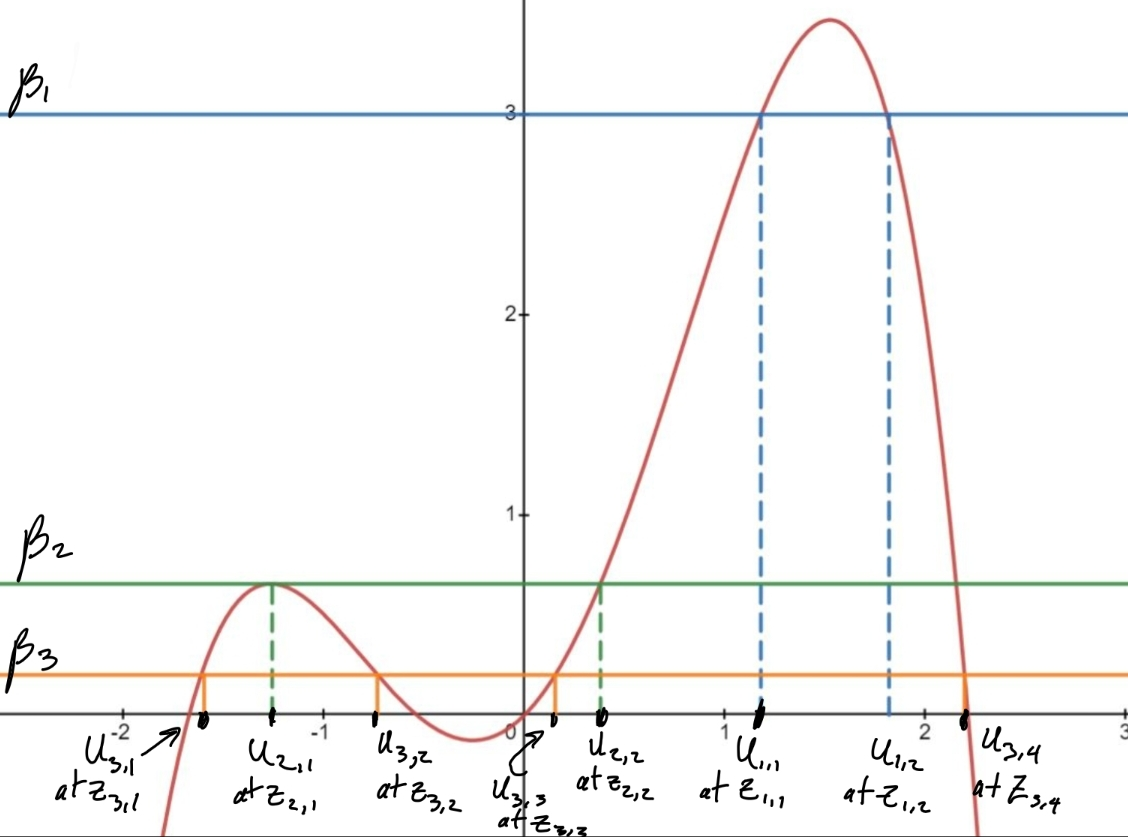
\includegraphics[width=.6\textwidth]{plots/4b-1.jpg}
        \end{center}
        Observe that various $\beta$ values have been plotted that show different maximum potential energy. 
        
        \noindent
        Let's begin by looking at the $\beta_1$ case. In this case there two real valued solutions classes, an elevation solitary wave with $U \in (-\infty, U_{1,1}]$ (seen below to the left) and another elevation solitary wave with $U \in [U_{1,2}, \infty)$ (seen to the right). In both cases it takes a finite amount of time to reach $U_{1,1}$ and $U_{1,2}$.
        \begin{center}
            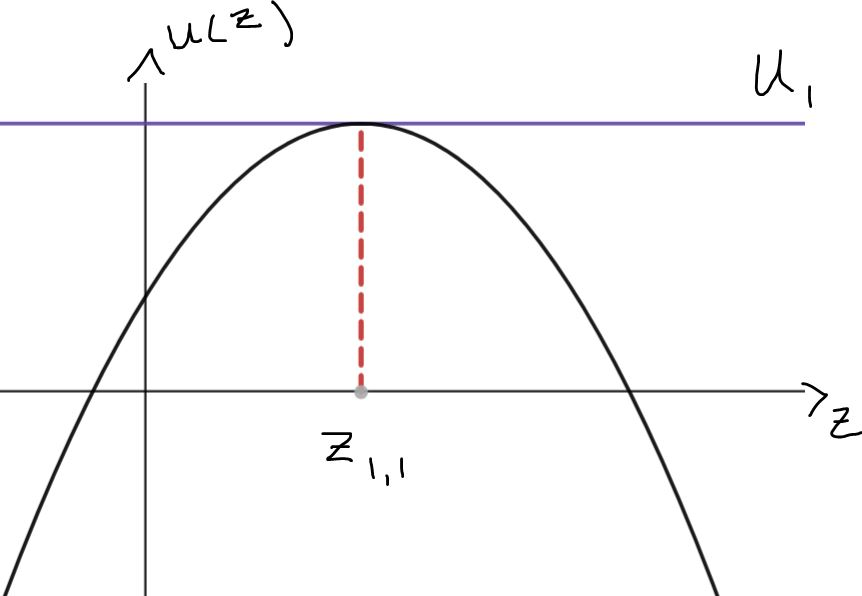
\includegraphics[width=.4\textwidth]{plots/4b-2.JPG}
            \qquad
            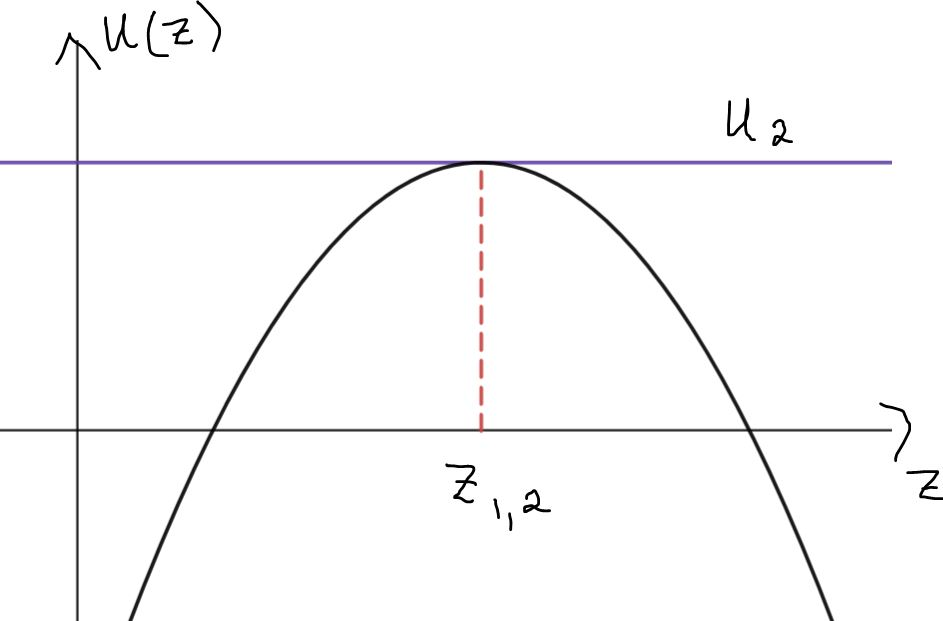
\includegraphics[width=.4\textwidth]{plots/4b-3.JPG}
        \end{center}

        \noindent
        Next let's look at the $\beta_2$ case. There are three real valued solution classes. A solitary solution with $U \in (-\infty,U_{2,1})$ (left), an elevation solitary wave with $U \in (U_{2,1},U_{2,2}]$ (right), and an elevation solitary wave with $U \in [U_{2,3}, \infty)$ (below). In these cases, it takes an infinite amount of time to reach $U_{2,1}$ since it is at a horizontal asymptote while $U_{2,2}$ and $U_{2,3}$ take a finite amount of time to reach.

        \begin{center}
            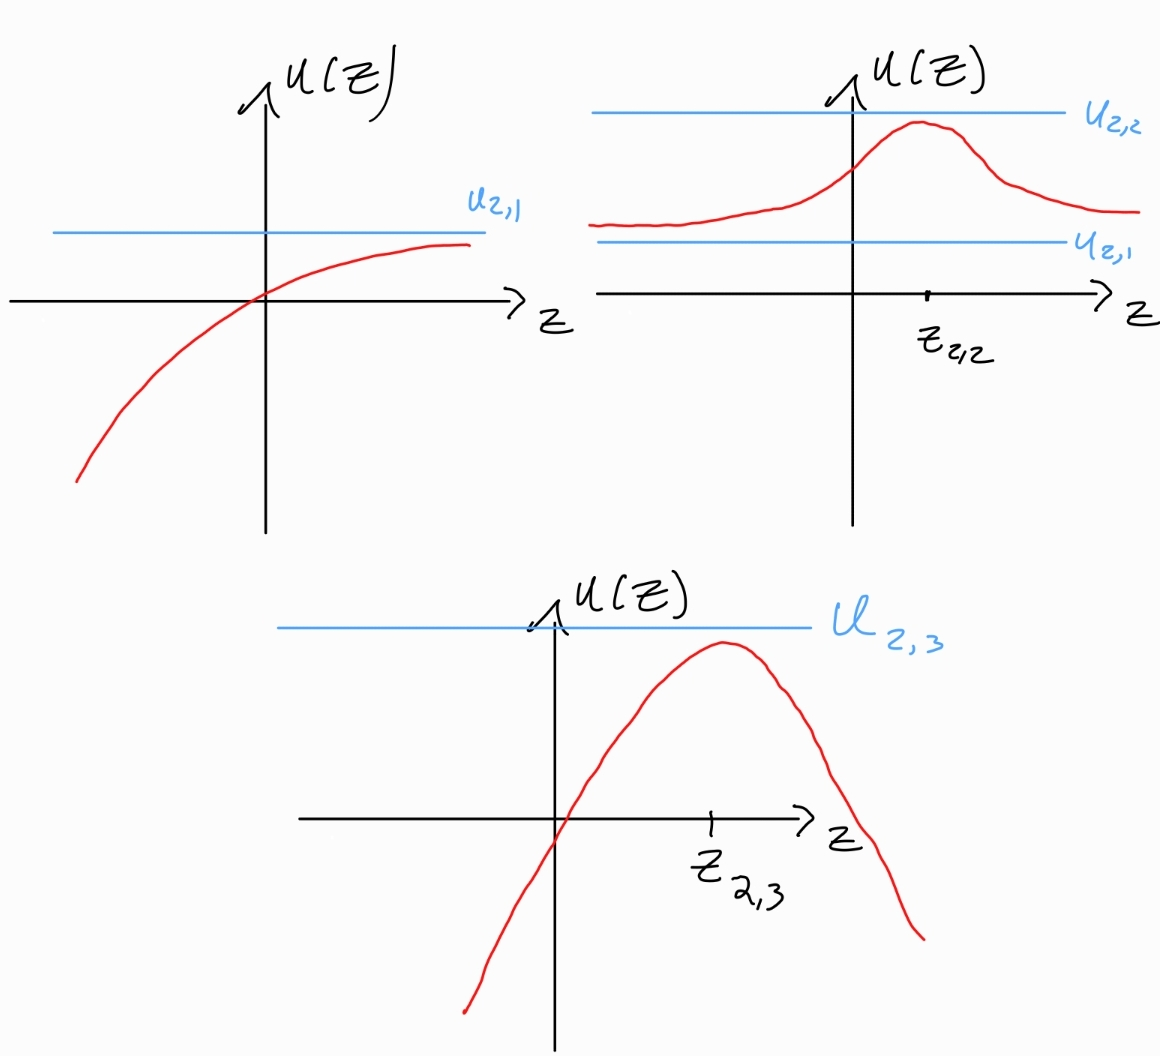
\includegraphics[width=.6\textwidth]{plots/4b-set1.jpg}
        \end{center}

        \noindent
        Next let's look at the $\beta_3$ case. There are three real valued solution classes. One is a solitary elevation wave with $U \in (-\infty, U_{3,1}]$ (left), one is a periodic wave with $U \in [U_{3,2},U_{3,3}]$ (right), and one is a solitary wave with $U \in [U_{3,4},\infty]$ (below). Note that it takes a finite amount of time to each all points $U_{3,1}, \cdots, U_{3,4}$.

        \begin{center}
            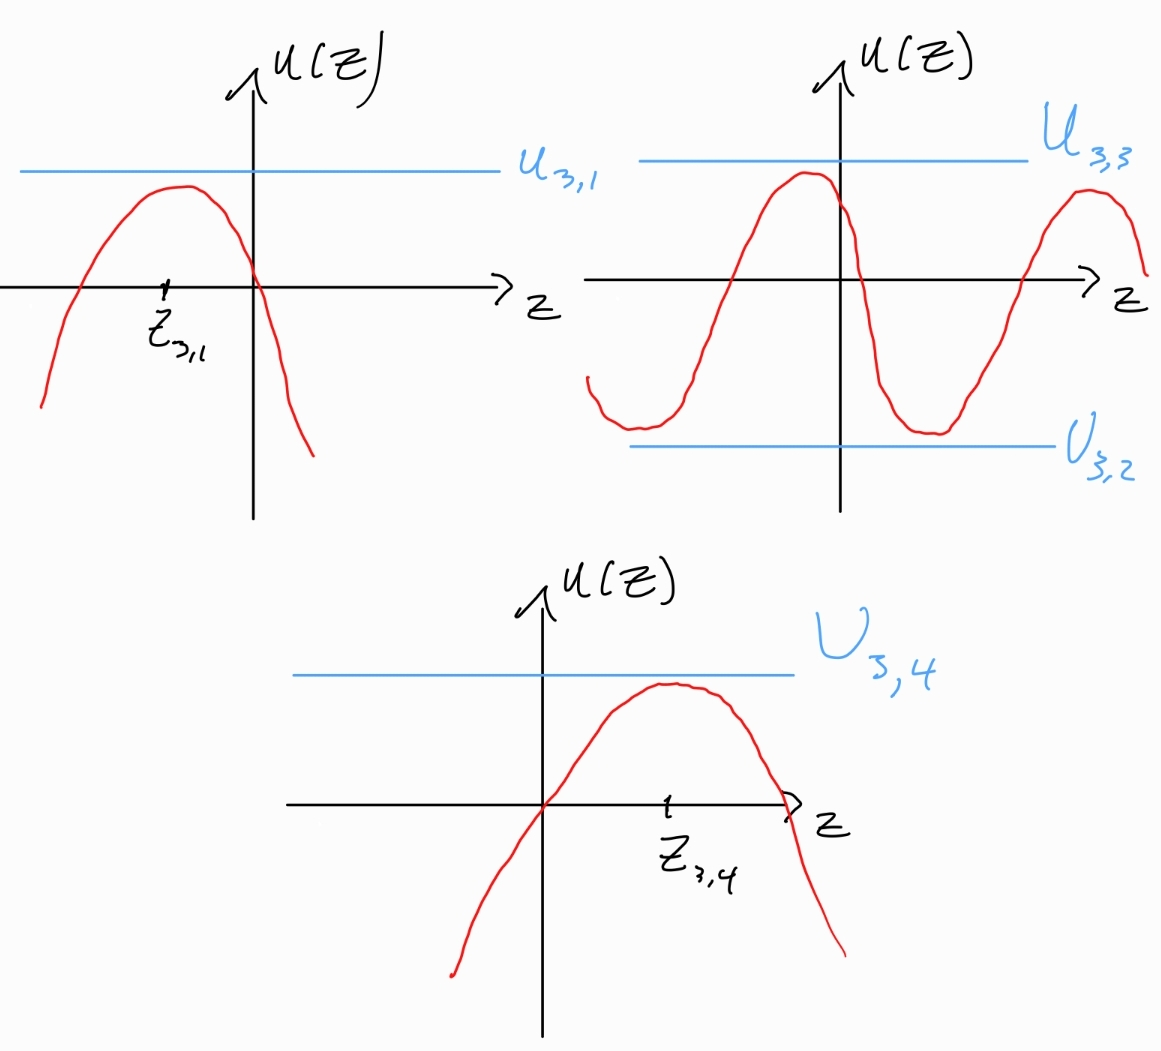
\includegraphics[width=.6\textwidth]{plots/4b-set2.jpg}
        \end{center}

        \noindent
        Finally let's consider the case when $\alpha = 0$. This results in a symmetric solution since both local maximum are at equal heights as seen in the following graph.
        \begin{center}
            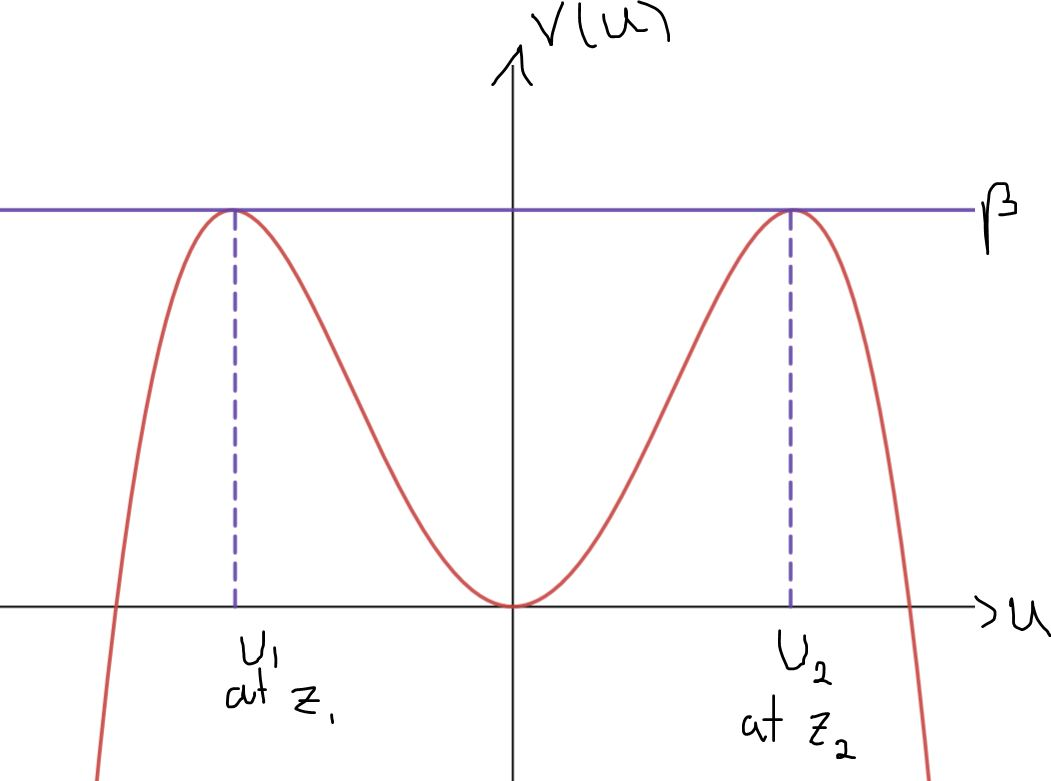
\includegraphics[width=.6\textwidth]{plots/4b-sym.jpg}
        \end{center}
        In this $\beta$ case there are three solution classes. One is a solitary wave with $U \in (-\infty, u_1)$ (left), one is a shock with $U \in (U_1,U_2)$ (right), and one is a solitary wave with $U \in (U_2, \infty)$ (below). Here it takes an infinite amount of time to reach $U_1$ and $U_2$.

        \begin{center}
            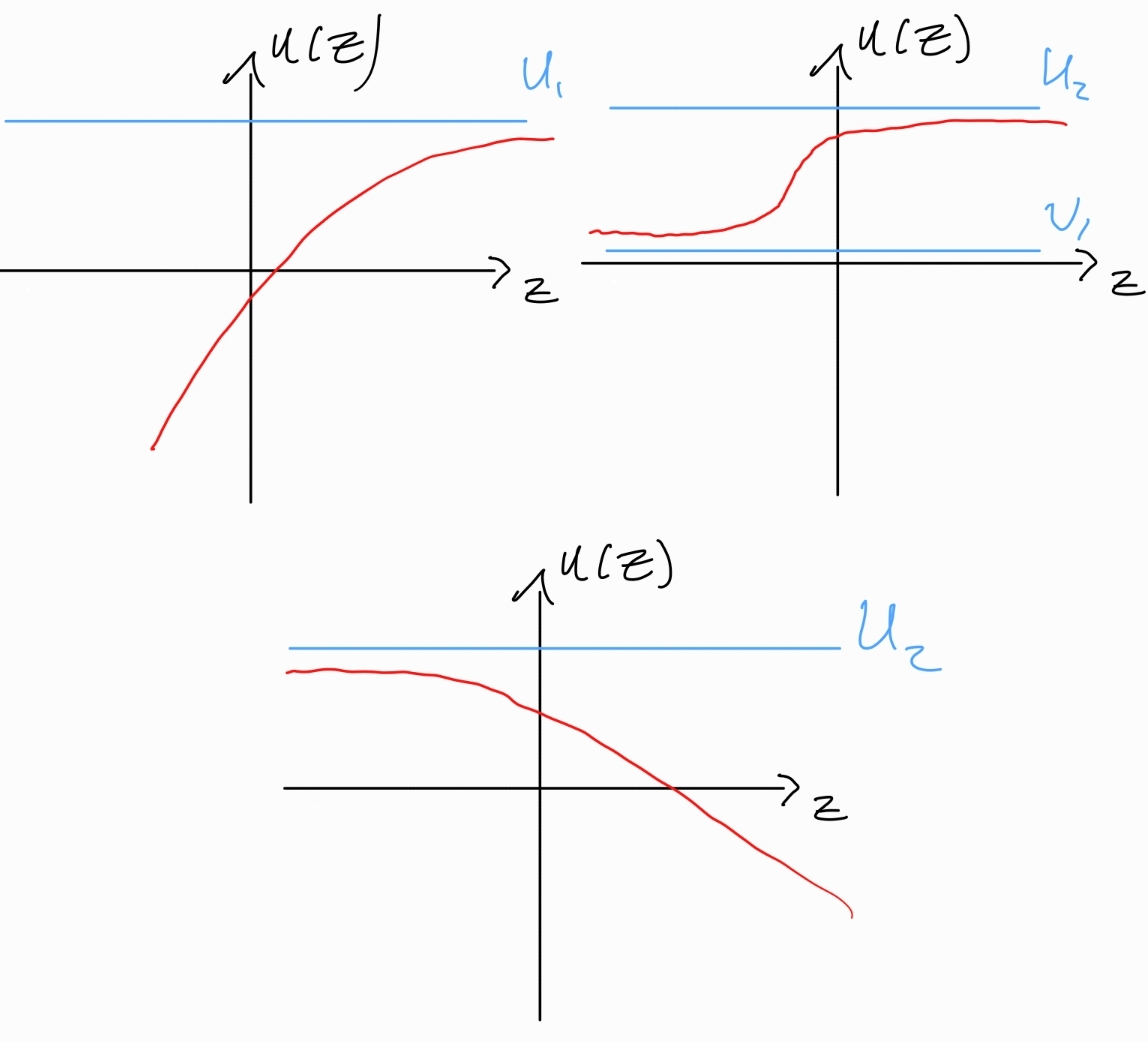
\includegraphics[width=.6\textwidth]{plots/4b-set3.jpg}
        \end{center}

        \noindent
        Next let's consider phase plane analyses. Recall that we found
        \[ 
            -4vU = -2U^3 + U'' + \alpha \implies U'' = -4vU + + 2U^3 - \alpha.
        \]
        If we let $u_1 = U$ and $u_2 = U'$ then we get the system
        \begin{align*}
            u_1' &= u_2\\
            u_2 &= -4vu_1 + 2u_1^3 - \alpha = -\pp{V(u_1)}{u_1},
        \end{align*}
        where $V(u) = \alpha u + 2vu^2 - \half u^4$. Thus we have a ODE dynamical system and we see that the equilibrium will have solutions of the form of the critical points of the potential equation
        \[ 
            \pp{v}{u} = -2U^3 + 4vU + \alpha = 0.
        \]
        Since this is a cubic equation with real coefficients we will always have at least one real root. To find the cases, recall that the discriminant is given by,
        \begin{align*}
            \Delta &= -4ac^3 - 27a^2d^2 = 512v^3 - 108\alpha^2.
        \end{align*}
        So when $\Delta > 0$ there will be two potential hills and one well (3 equilibrium points), let's call this case 3. When $\Delta \to 0$, one potential hill goes away, leaving a horizontal tangent (2 equilibrium points), let's call this case 2. And When $\Delta < 0$ there will be one potential hill (1 equilibrium point), let's call this case 1. Each of the cases can be seen in the following graphs where $v=1$ and $\alpha =1$.   
        \begin{center}
            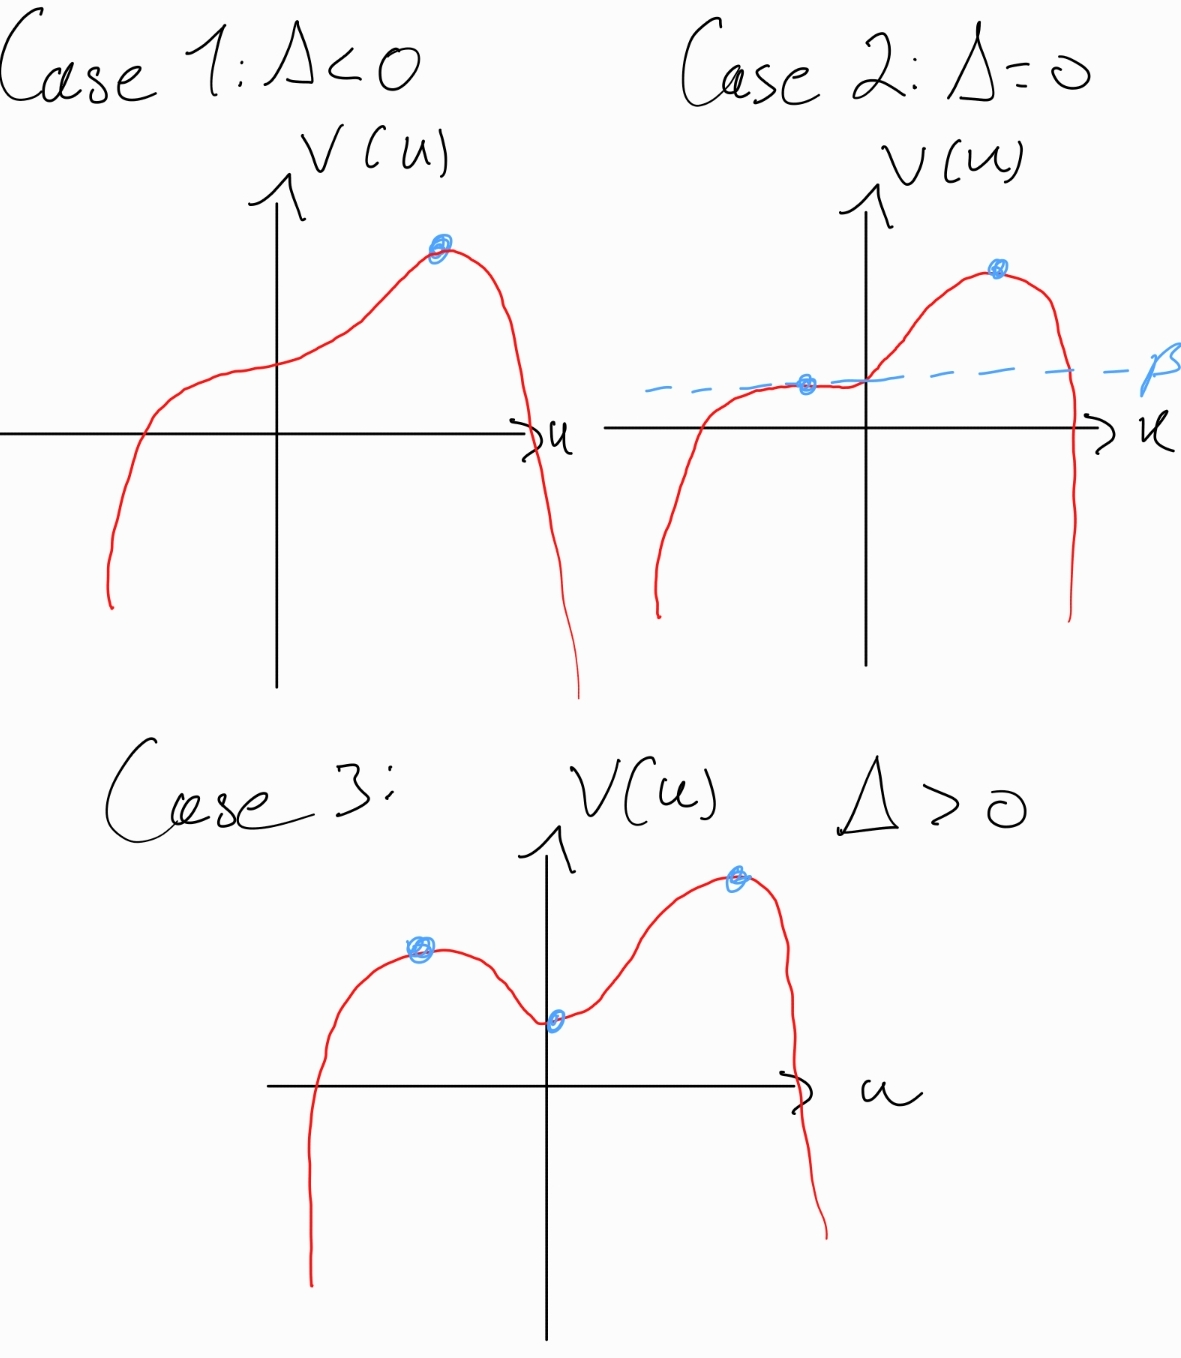
\includegraphics[width=.6\textwidth]{plots/4b-situations.jpg}
        \end{center}

        \noindent 
        Let's consider case 1: $\Delta < 0$. In this case we expect to find that all solutions move away from the equilibrium position since it is a hill. Letting $\alpha = 1$ and $v=1$ we can see that the phase potrait looks like the following phase plane.

        \begin{center}
            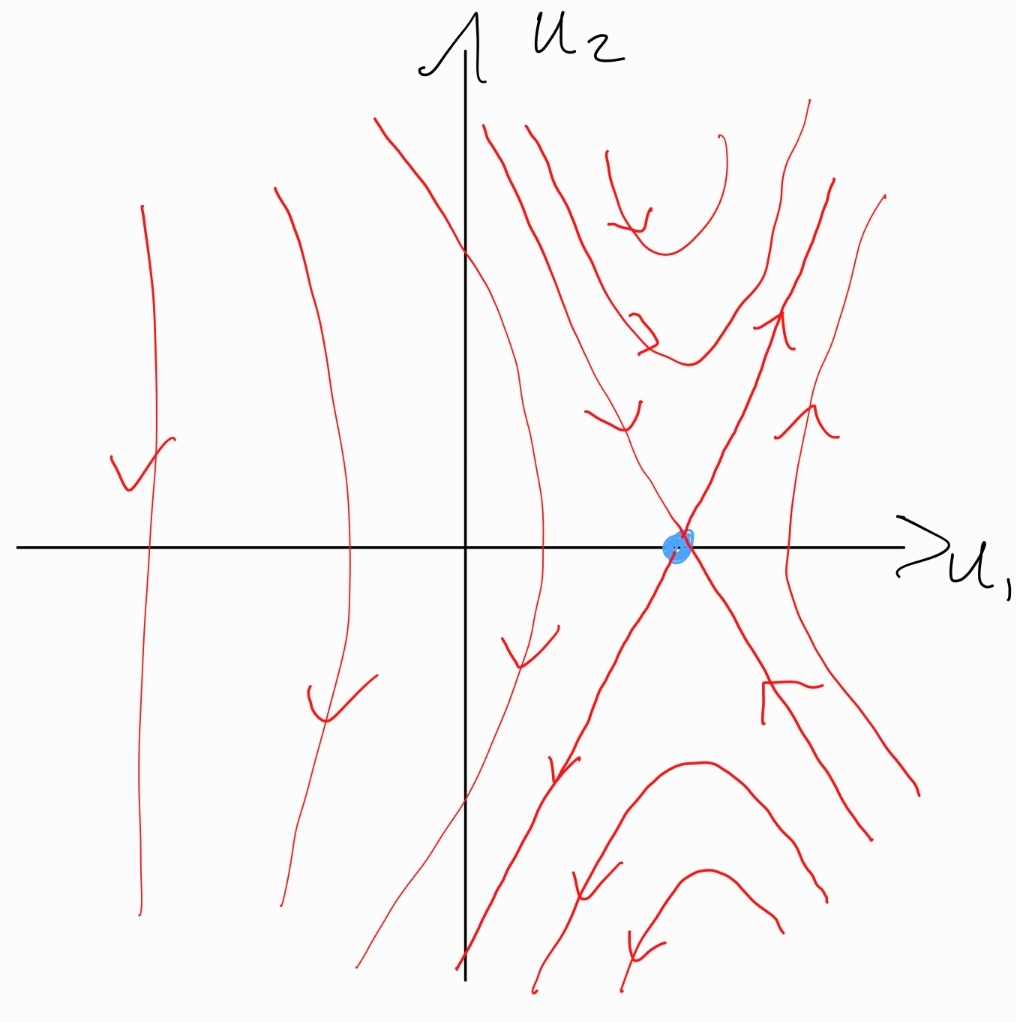
\includegraphics[width=.6\textwidth]{plots/4b-phase1.jpg}
        \end{center}        

        \noindent 
        Let's consider case 2: $\Delta = 0$. For $\Delta = 0$, let $\alpha = 1$ and then $v = \frac{3}{4(2)^{\frac{3}{2}}}$. We expect to have similar behavior as before around the maximum critical points but we also have a horizontal tangent critical point which degenerates. Thus we come up with the following phase plane.

        \begin{center}
            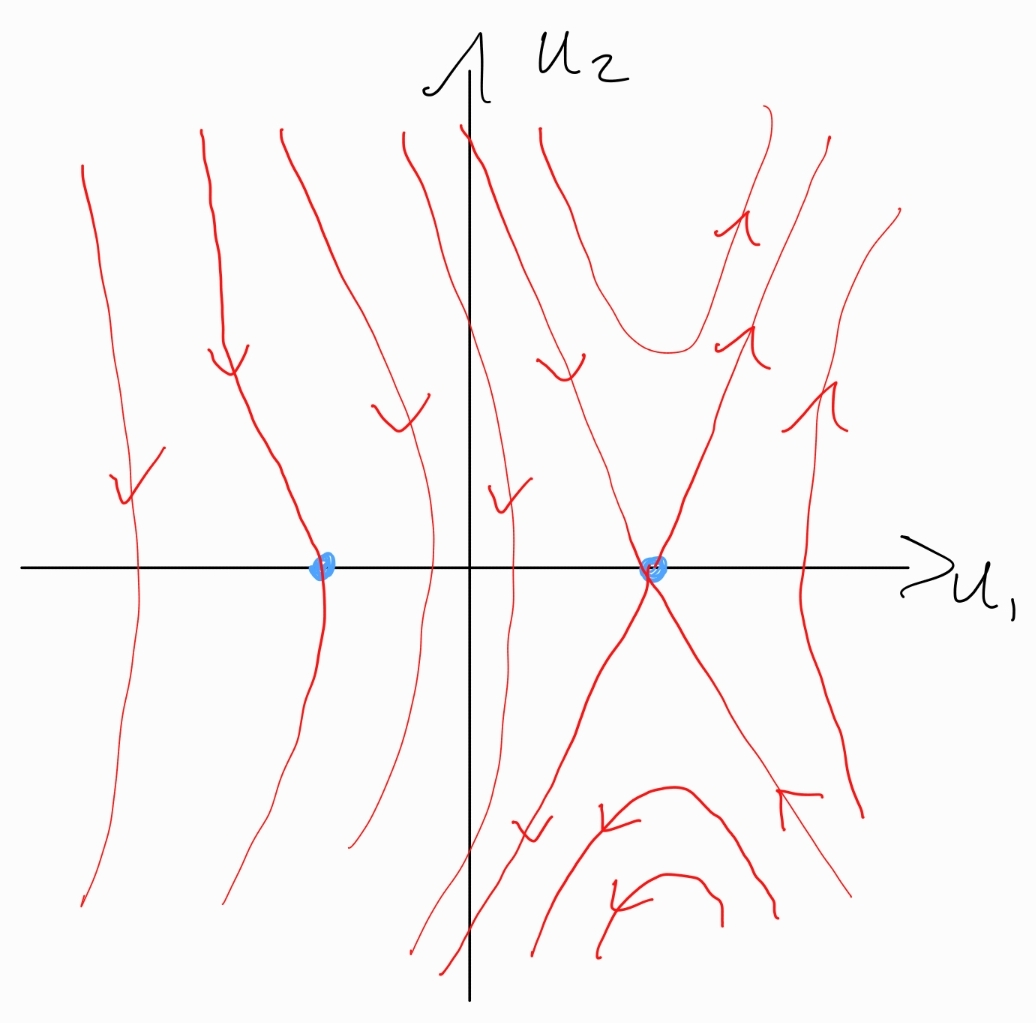
\includegraphics[width=.6\textwidth]{plots/4b-phase2.jpg}
        \end{center}

        \noindent 
        Let's consider case 3: $\Delta > 0$. In this case, there will be two different scenarios. One where the local maximum critical points are not equal (i.e. $\alpha \neq 0$) and the other where the local maximum are at equal heights (i.e. $\alpha = 0$). Let's first consider when maximum are unequal. Let's let $v=1$ and $\alpha = 1$. We expect solutions on the outer side of the hills to run to infinity while there is a different behavior around the well between the hills. We noted before that the well will have periodic solutions and thus we expect a center type critical point. Note that we can observe a homoclinic orbit at the left hill. 

        \begin{center}
            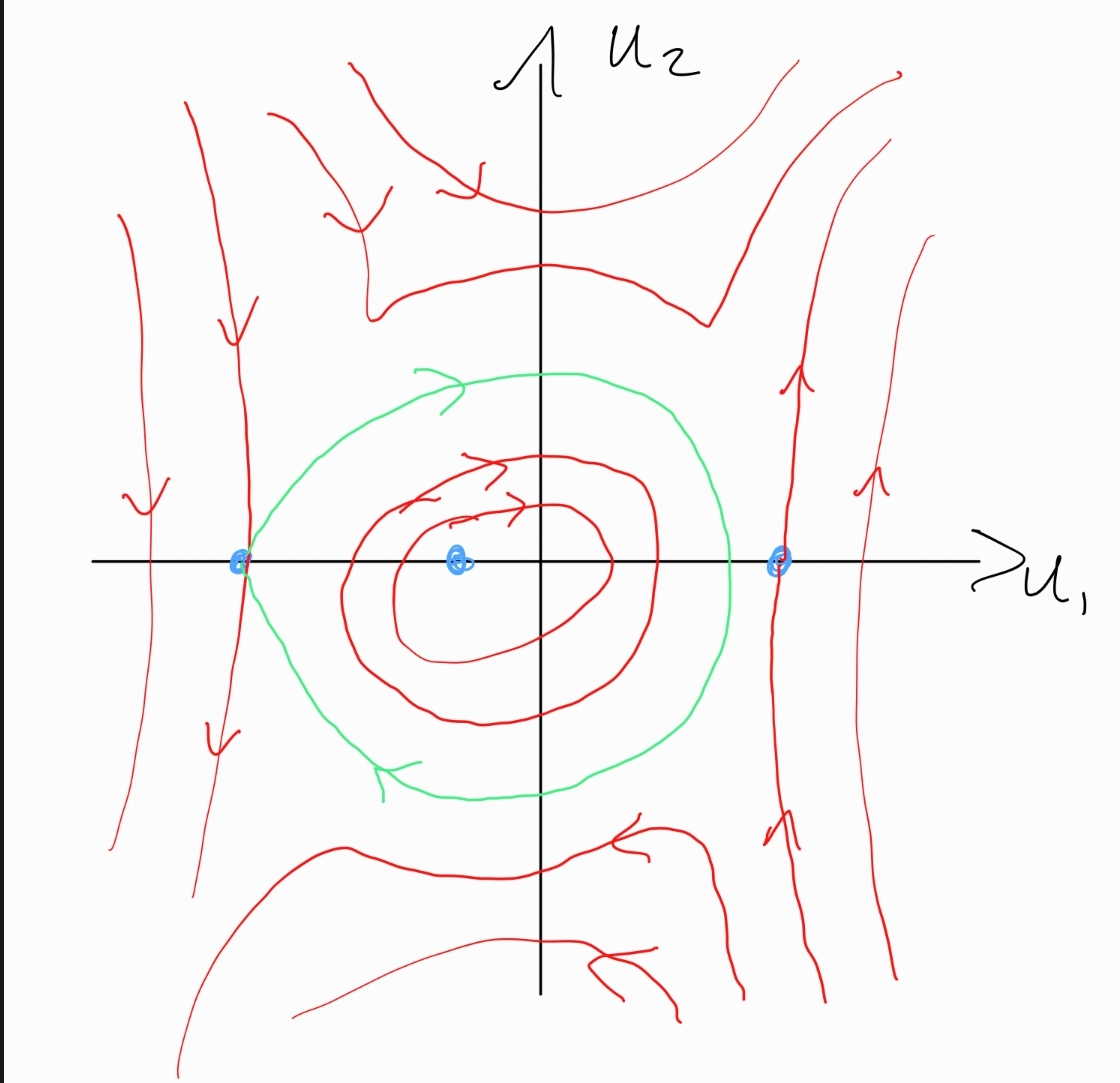
\includegraphics[width=.6\textwidth]{plots/4b-phase3.jpg}
        \end{center}

        Now consider the scenario where $\alpha =0$ and let $v=1$. In this case we have similar behavior as before except a heteroclinic orbit arises between the two hills. This correlates with the previous observation we made of when $\alpha = 0$ a shock wave arises rather than a periodic wave.  
        
        \begin{center}
            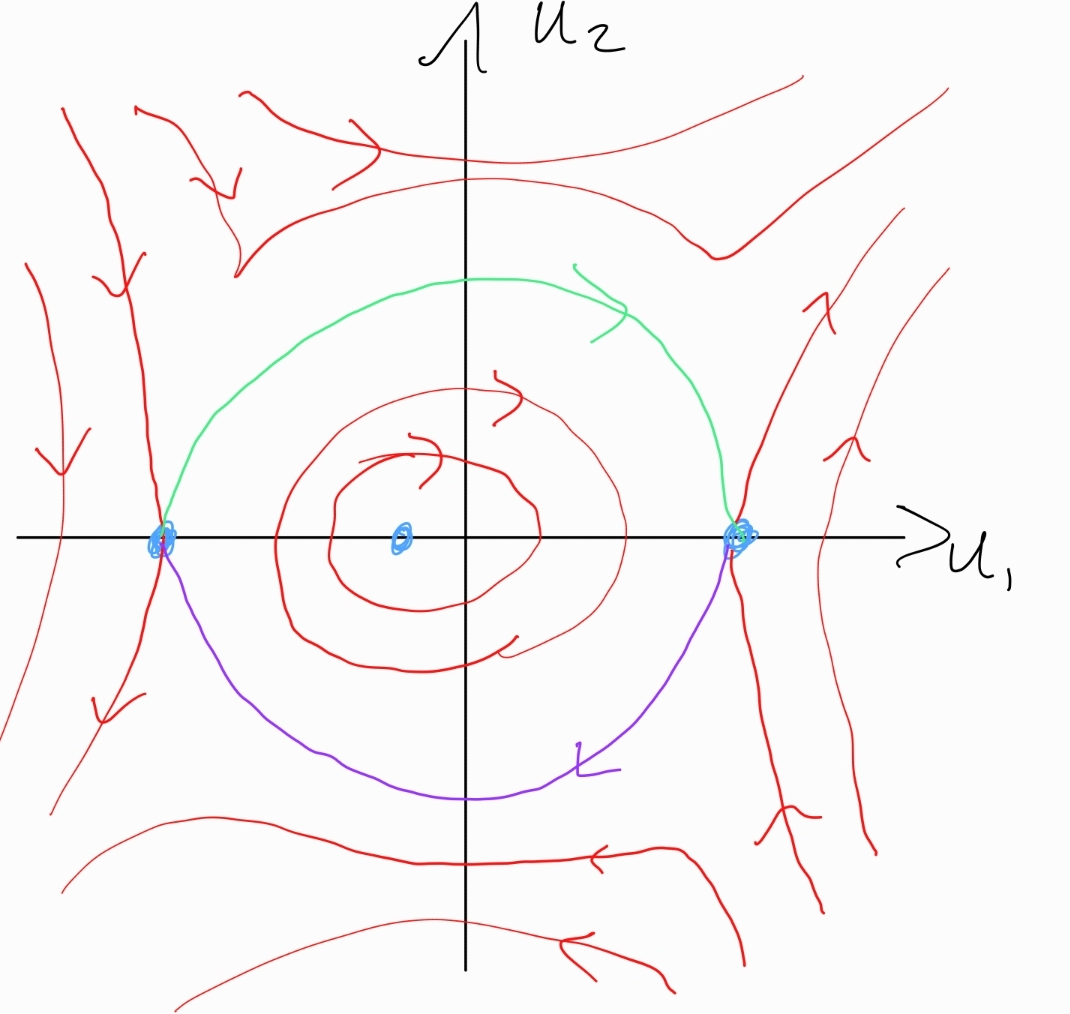
\includegraphics[width=.6\textwidth]{plots/4b-phase4.jpg}
        \end{center}

        \item[{\bf b.}]
        Now we want to obtain the explicit functional form of the solution. Recall the potential energy equation,
        \[ 
            \frac{1}{2}U'^2 + V(u) = \beta,
        \]
        which we can solve to get
        \[
            u' = \pm \sqrt{2(\beta - V(u))}.
        \]
        Now we can separate variables to get an implicit solution 
        \[
            \pm\int_{u_0}^u \frac{du}{\sqrt{2(\beta - V(u))}} = \pm \int_0^zdz = \pm z.
        \]
        Thus we have obtained the implicit solution to be,
        \[
            \pm z = \int_{u_0}^u \frac{du}{\sqrt{2(\beta - V(u))}}.
        \]
        Now we will not consider the homoclinical case but rather focus on the heteroclinical case. The heteroclinical case only occurs when $V$ is symmetric and the local maximums are equal, i.e. when $\alpha = 0$. Thus the potential energy function reduces to
        \[
        V(u) = 2vu^2 - \frac{1}{2}u^4. 
        \]
        To find the maximum height, consider that
        \begin{align*}
            \pp{v}{u} = 4vU - 2u^3 = 0 \implies u^2 = 2v \implies u = \pm \sqrt{2v}.
        \end{align*}
        By definition of the heteroclinic orbit, we know that $u \to \pm \sqrt{2v}$ as $x \to \pm \infty$. We also note that all derivatives of $u$ are to zero as $x \to \infty$. Knowing these facts we can now solve for the value of $\beta$ by solving the equation
        \begin{align*}
            -2vU^2 &= \frac{-U^4}{2} + \frac{U'^2}{2} + \alpha U - \beta\\
            \implies -2v(2v) &= \frac{-4v^2}{2} - \beta\\
            \implies \beta &= 2v^2.
        \end{align*}
        We are now able to further evaluate our implicit integral using that $\alpha = 0$ and $\beta = 2v^2$
        \begin{align*}
            \pm z &= \int_{u_0}^u \frac{du}{\sqrt{2(\beta - V(u))}}\\
            \pm z &= \int_{u_0}^u \frac{du}{\sqrt{2(2v^2 + \frac{1}{2}u^4 - 2vU^2)}}\\
            \pm z &= \int_{u_0}^u \frac{du}{\sqrt{4v^2 + U^4 - 4vU2}}.\\
        \end{align*}
        Using Mathematica to compute this integral we get
        \begin{align*}
            \pm z &= - \frac{1}{\sqrt{2v}}\tanh^{-1}\paren{\frac{u}{\sqrt{2v}}} |_{u_0}^u\\
            &= -\frac{1}{2v}\paren{\tanh^{-1}\paren{\frac{u}{\sqrt{2v}}}-\tanh^{-1}\paren{\frac{u_0}{\sqrt{2v}}}}.
        \end{align*}
        We can now solve for $u$ as follows
        \begin{align*}
            -\frac{1}{2v}\paren{\tanh^{-1}\paren{\frac{u}{\sqrt{2v}}}} &= \pm z -  \frac{1}{2v}\paren{\tanh^{-1}\paren{\frac{u_0}{\sqrt{2v}}}}\\
            \tanh^{-1}\paren{\frac{u}{\sqrt{2v}}} &= \mp \sqrt{2v} z -  \tanh^{-1}\paren{\frac{u_0}{\sqrt{2v}}}\\
            \frac{u}{\sqrt{2v}} &= \tanh\paren{\mp \sqrt{2v} z -  \tanh^{-1}\paren{\frac{u_0}{\sqrt{2v}}}}\\
            u &= \sqrt{2v}\tanh\paren{\mp \sqrt{2v} z -  \tanh^{-1}\paren{\frac{u_0}{\sqrt{2v}}}},\\
        \end{align*}
        and if we let $\tanh^{-1}\paren{\frac{u_0}{\sqrt{2v}}} = -\sqrt{2v}x_0$ we get that
        \[
            u(x,t) = \sqrt{2v}\tanh(\mp\sqrt{2v}z - \sqrt{2v}x_0) = \sqrt{2v}\tanh(\sqrt{2v}(\mp z - x_0)). 
        \]
        Recalling that we let $u(x,t) = U(x-vt)$, we have found an explicit solution for the heteroclinic orbit to be
        \[
            u(x,t) = \sqrt{2v}\tanh(\sqrt{2v}(x - x_0 \mp v t)).
        \]
    \end{enumerate}
\end{solution}

%----------------------------------------------------------------------------------------------------%
%\vskip 20pt
\newpage

%---------------%
%---Problem 5---%
%---------------%

%--status--$

\begin{problem}
    Consider the so-called Derivative NLS equation (DNLS)
$$
b_t+\alpha \left(b |b|^2\right)_x-i b_{xx}=0.
$$
This equation arises in the description of quasi-parallel waves in space plasmas. Here $b(x,t)$ is a complex-valued function.
\begin{enumerate}

\item[{\bf a.}] Using a polar decomposition
$$
b(x,t)=B(x,t)e^{i\theta(x,t)},
$$
with $B$ and $\theta$ real-valued functions, and separating real and imaginary parts (after dividing by the exponential), show that you obtain the system
\begin{align*}
B_t+3\alpha B^2 B_x+\frac{1}{B}(B^2 \theta_x)_x&=0,\\
\theta_t+\alpha B^2 \theta_x+\theta_x^2-\frac{1}{B}B_{xx}&=0.
\end{align*}

\item[{\bf b.}] Assuming a traveling-wave envelope, $B(x,t)=R(z)$, with $z=x-vt$  and constant $v$, show that $\theta(x,t)=\Phi(z)-\Omega t$, with constant $\Omega$, is consistent with these equations. You can show (but you don't have to) that assuming a traveling-wave amplitude results in only this possibility for $\theta(x,t)$. At this point, we have reduced the problem of finding solutions with traveling envelope to that of finding two one-variable functions $R(z)$ and $\Phi(x)$. The problem also depends on two parameters $v$ (envelope speed) and $\Omega$ (frequency like).

\item[{\bf c.}] Substituting these ansatz in the first equation of the above system, show that
\[
\Phi'=\frac{C+vs-3s^2}{2s},
\]
where $C$ is a constant and $s=\alpha R^2/2$.

\item[{\bf d.}] Lastly, by substituting your results in the second equation of the system, show that $s(z)$ satisfies
\[
\frac{1}{2}s'^2+V(s)=E,
\]
the equation for the motion of a particle with potential $V(s)$. Find the expression for $V(s)$ and for $E$.

\end{enumerate}

You can (don't do this; it would take a lot of work; there's a lot of cases) use this observation to classify the traveling-envelope solutions of the DNLS, in the same vein that we did at the beginning of this chapter for KdV.

\end{problem}

\begin{solution}
   
    \noindent
    Consider the so-called Derivative NLS equation (DNLS)
    \[
    b_t+\alpha \left(b |b|^2\right)_x-i b_{xx}=0.
    \]
    
    \begin{enumerate}
        \item[{\bf a.}]
        Let's begin by using a polar decomposition
        \[
            b(x,t) = B(x,t)e^{i\theta(x,t)},
        \]
        where $B$ and $\theta$ are real-valued functions. First let's find the partials
        \begin{align*}
            b_t &= B_te^{i\theta} + Bi\theta_te^{i\theta}\\
            b_x &= B_xe^{i\theta} + Bi\theta_xe^{i\theta}\\
            b_{xx} &= b_{xx}e^{i\theta} + B_x i \theta_x e^{i\theta} + B_xi\theta_xe^{i\theta} + Bi\theta_{xx}e^{i\theta} - B\theta_x^2e^{i\theta}.
        \end{align*}
        Plugging these into the DNLS equation we get
        \begin{align*}
            B_te^{i\theta} + Bi\theta_te^{i\theta} + \alpha(Be^{i\theta}B^2)_x - i\paren{b_{xx}e^{i\theta} + B_x i \theta_x e^{i\theta} + B_xi\theta_xe^{i\theta} + Bi\theta_{xx}e^{i\theta} - B\theta_x^2e^{i\theta}} &= 0.\\
        \end{align*}
        Expanding this equation and dividing out the exponential we obtain
        \begin{align*}
            B_t + B\theta_t i + \alpha i B^3\theta_x + \alpha 3 B^2B_x - iB_{xx} + B_x\theta_x + B_x\theta_x + B\theta_{xx} + iB\theta_x^2 = 0.
        \end{align*}
        Taking the real part of this equation gives
        \begin{align*}
            B_t + 3\alpha B^2 B_x + 2B_x \theta_x + B\theta_{xx} &= 0\\
            B_t + 3\alpha B^2 B_x + \frac{1}{B}(B^2\theta_x)_x &= 0.
        \end{align*}
        Next let's look at the imaginary part
        \begin{align*}
            B\theta_t + \alpha B^3 \theta_x + B_{xx} + B\theta_x^2 &= 0\\
            \theta_t + \alpha B^2 \theta_x + \frac{1}{B}B_{xx} + \theta_x^2 &= 0.
        \end{align*}
        Thus we get the system,
        \begin{align}
            B_t+3\alpha B^2 B_x+\frac{1}{B}(B^2 \theta_x)_x&=0,\\
            \theta_t+\alpha B^2 \theta_x+\theta_x^2-\frac{1}{B}B_{xx}&=0.
        \end{align}

        \item[{\bf b.}]
        Now let's assume a traveling-wave envelope, $B(x,t) = R(z)$ with $z = x - vt$ and constant $v$. Let $\theta(x,t) =\Phi(z) + \Omega t$. Now let's find the partials
        \begin{align*}
            \theta_t &= \pp{\theta}{z}\pp{z}{t} + \pp{\theta}{t} = -v\Phi_z - \Omega\\
            \theta_x &= \pp{\theta}{z}\pp{z}{x} = \Phi_z\\
            B_t &= \pp{R}{z}\pp{z}{t} = -vR_z\\
            B_x &= \pp{R}{z}\pp{z}{x} = R_z.
        \end{align*}
        Plugging these into the system formed by (18) and (19) we get
        \begin{align*}
            -vR_z + 3 \alpha R^2R_z + \frac{1}{R}\paren{R^2\Phi_z}_z &= 0\\
            -v\Phi_z - \Omega + \alpha R^2\Phi_z + \Phi_z^2 - \frac{1}{R}R_{zz} &= 0.
        \end{align*}
        We can see that these equations form an ODE that is only dependent on $z$ (i.e. there is no $t$ or $x$ dependence) and thus we have shown that $\theta(x,t) =\Phi(z) + \Omega t$ is consistent with our equations.


        \item[{\bf c.}]
        Now substituting our ansatz into (18) gives
        \begin{align*}
            0 &= -vR' + 3\alpha R^2 R_x + \frac{1}{R}(R^2 \Phi')_x\\
            (R^2 \Phi')_x &= vRR' - 3 \alpha R^3 R'\\
            R^2 \Phi' &= \int vRR'- 3 \alpha R^3 R'dx\\
            R^2 \Phi' &=  \frac{v}{2}R^2 - \frac{3\alpha}{4}R^4 + C_1,
        \end{align*}
        where $C_1$ is a constant from integration. Now if we let $s = \frac{\alpha R^2}{2}$ that means that $R^2 = \frac{2s}{\alpha}$. Thus we have,
        \begin{align*}
            \frac{2s}{\alpha}\Phi' &= \frac{v}{2}\frac{2s}{\alpha} - \frac{3\alpha}{4} \frac{4s^2}{\alpha^2} + C_1\\
            \frac{2s}{\alpha}\Phi' &= \frac{vs}{\alpha} - \frac{12s^2}{4\alpha} + C_1\\
            2s \Phi' &= vs - 3s^2 + \alpha C_1\\
            \Phi' &= \frac{vs - 3s^2 + C}{s2},
        \end{align*}
        where $C = \alpha C_1$ is a constant.

        \item[{\bf d.}]
        Recall from part b that we found,
        \begin{align}
            -v\Phi' - \Omega + \alpha R^2\Phi' + \Phi'^2 - \frac{1}{R}R_{zz} = 0.
        \end{align}
        Now let $-v\Phi_z - \Omega + \alpha R^2\Phi_z + \Phi_z^2 = G(z)$. Since $G(z)$ is only in terms of $z$ and since $s$ is only a function of $z$ we can set
        \[
            -v\Phi' - \Omega + \alpha R^2\Phi' + \Phi'^2 = G(z) = F'(s).
        \]
        Thus we can rewrite (20) as
        \[
            F'(s) - \frac{R''}{R} = 0,
        \]        
        and multiplying by $s'$ we get
        \[
            F'(s)s' - \frac{R''}{R}s' = 0.
        \]
        Noting that $s = \frac{\alpha R^2}{2} \implies s'=\frac{2RR'\alpha}{2} = RR'\alpha$ we get 
        \begin{align*}
            F'(s)s' - \frac{R''}{R}RR' &= 0\\
            (F(s))' - R'R'' &= 0\\
            (F(s))' - \paren{\frac{R'^2}{2}}' &= 0\\
            F(s) - \frac{R'^2}{2} &= 0\\
            F(s) - \frac{s'^2/\alpha R^2}{2} &= 0\\
            F(s) - \frac{s'^2}{s} &= 0.
        \end{align*}
        Thus we have that
        \begin{align}
            F(s) - \frac{s'^2}{s} &= 0.
        \end{align}
        Next consider that
        \begin{align*}
            F'(s) &= -v\Phi' - \Omega + \alpha R^2\Phi' + \Phi'^2\\
            &= -v \paren{\frac{c + vs - 3s^2}{2s}} - \Omega + 2s\paren{\frac{c + vs - 3s^2}{2s}} + \paren{\frac{c + vs - 3s^2}{2s}}^2\\
            &= -\frac{v}{2}s^{-1}\paren{c + vs - 3s^2} - \Omega + c + vs - 3s^2 + \frac{1}{4}s^{-2}\paren{c + vs - 3s^2}\paren{c + vs - 3s^2}\\
            &=-\frac{v}{2}cs^{-1} - \frac{1}{2}v^2 + \frac{3}{2}vs - \Omega + c + vs - 3s^2 + \frac{1}{4}c^2s^{-2} + \frac{1}{4}cvs^{-1} - \frac{3}{4}c\\ 
            &+ \frac{1}{4}cvs^{-1} + \frac{1}{4}v^2 - \frac{3}{4}vs - \frac{3}{4}c - \frac{3}{4}vs + \frac{9}{4}s^2\\
            &= -\frac{3}{4}s^2 + vs + \frac{1}{4}c^2s^{-2} - \Omega - \frac{1}{2}c - \frac{1}{4}v^2.
        \end{align*}
        Now if we integrate $F'(s)$
        \[
            F(s) = - \frac{1}{4}s^3 + \frac{v}{2}s^2 - \frac{1}{4}c^2s^{-1}- \paren{\Omega + \frac{1}{2}c + \frac{1}{4}v^2}s + \delta,
        \]
        where $\delta$ is an integration constant. Plugging $F(s)$ into (21) gives
        \begin{align*}
            - \frac{1}{4}s^3 + \frac{v}{2}s^2 - \frac{1}{4}c^2s^{-1}- \paren{\Omega + \frac{1}{2}c + \frac{1}{4}v^2}s + \delta - \frac{s'^2}{s} &= 0\\
            -\frac{1}{2}s^4 + vs^3 - \frac{c^2}{2} - \paren{2\Omega + c + \frac{1}{2}v^2}s^2 - 2\delta s &= \frac{-c^2}{2}\\
            \frac{1}{2}s'^2 + \frac{1}{4}s^4 - vs^3 + \paren{2\Omega + c + \frac{1}{2}v^2}s^2 - 2\delta s &= \frac{-c^2}{2}.\\
        \end{align*}
        Thus if we let $V(s) = \frac{1}{2}s^4 - vs^3 + \paren{2\Omega + c + \frac{1}{2}v^2}s^2 - 2\delta s$ and $E = \frac{-c^2}{2}$ we have shown that $s(z)$ satisfies
        \[
            \frac{1}{2}s'^2 + V(s) = E.
        \]

    \end{enumerate}
\end{solution}

%----------------------------------------------------------------------------------------------------%
%\vskip 20pt
\newpage

%---------------%
%---Problem 6---%
%---------------%

%--status--$

\begin{problem}
    Consider example 5.2 in the notes. Check that $y=x^2/t$ and $t^{1/2} q$ are both scaling invariant. Find the ordinary differential equation satisfied by $G(y)$, for similarity solutions of the form $q(x,t)=t^{-1/2}G(y)$. Show that this results in the same similarity solutions as in the example.
\end{problem}

\begin{solution}

    \noindent
    Consider nonlinear Schr\"odinger (NLS) equation,
    \[ 
        i q_t = -q_{xx} + \sigma \abs{q}^2q.
    \]
    First let's verify that both $y = x^2/t$ and $y = t^{1/2}q$ are scaling invariant. Recall that the scaling transformations are
    \[
        x = \frac{\hat{x}}{a}, ~~ t = \frac{\hat{t}}{b}, ~~ u=c\hat{u}.
    \]
    Then observe that
    \[
        y = \frac{x^2}{t} = \frac{\frac{\hat{x}^2}{a^2}}{\frac{\hat{t}^2}{a^2}} = \frac{\hat{x}^2}{\hat{t}},
    \]
    and
    \[
        y = t^{\frac{1}{2}}q = \paren{\frac{\hat{t}^\frac{1}{2}}{a^2}}\hat{q}a = \hat{t}^{\frac{1}{2}} \hat{q}.
    \]
    Thus we have verified that $y = x^2/t$ and $y = t^{1/2}q$ are scaling invariant. Imposing that the two scaling invariant groups are function of each other we get
    \[
        t^{\frac{1}{2}}g(x,t) = G(y) \implies g(x,t) = t^{-\frac{1}{2}}G(y) = t^{\-\frac{1}{2}}G\paren{\frac{x^2}{t}}.
    \]
    Let's compute the partials of $g(x,t)$
    \begin{align*}
        g_t &= \frac{1}{2}t^{-\frac{3}{2}}G(y) + t^{-\frac{1}{2}}G'(y)\paren{-\frac{x^2}{t^2}}\\
            &= -\frac{1}{2}t^{-\frac{3}{2}}G(y) - t^{-\frac{5}{2}}x^2G'(y)\\
        g_x &= t^{-\half}G'(y)(2 \frac{x}{t})\\
            &= 2t^{-\frac{3}{2}}xG'(y)\\
        g_{xx} &= 2t^{-\frac{3}{2}}G'(y) + 4t^{-\frac{5}{2}}x^2G''(y).
    \end{align*}
    Plugging these into the NLS equation
    \begin{align*}
        i\paren{-\frac{1}{2}t^{-\frac{3}{2}}G(y) - t^{-\frac{5}{2}}x^2G'(y)} &= -2t^{-\frac{3}{2}}G'(y) - 4t^{-\frac{5}{2}}x^2G''(y) + \sigma\abs{\paren{t^{-\half}G(y)}^2}t^{-\half}G(y)\\
        i\paren{-\frac{1}{2}t^{-\frac{3}{2}}G(y) - t^{-\frac{5}{2}}x^2G'(y)} &= -2t^{-\frac{3}{2}}G'(y) - 4t^{-\frac{5}{2}}x^2G''(y) + \sigma t^{-\frac{3}{2}}\abs{G(y)^2}G(y)\\
        i\paren{-\half t^{-\frac{3}{2}}G(y)-yt^{-\frac{3}{2}}G'(y)} &= -4yt^{-\frac{3}{2}}G''(y) - 2t^{-\frac{3}{2}}G'(y) + \sigma t^{-\frac{3}{2}}\abs{G(y)}^2G(y)\\
        i\paren{-\half G(y)-yG'(y)} &= -4yG''(y) - 2G'(y) + \sigma \abs{G(y)}^2G(y).\\
    \end{align*}
    Now if we $G(y) = \hat{G}(z)$ where $z = xt^{-\half}$, then we get $z = y^{\half}$. Computing the partials
    \begin{align*}
        G'(y) = \pp{\hat{G}(z)}{z}\pp{z}{y} &= \hat{G}'(z) \half y^{-\half}\\
        &= \frac{1}{2z}\hat{G}'(z)\\
        G''(y) = \pp{\frac{1}{2z}\hat{G}'(z)}{z}\pp{z}{y} &= -\frac{1}{4z^3}\hat{G}'(z) + \frac{1}{4z^{-2}}\hat{G}''(z).
    \end{align*}
    Plugging these into our NLS equation we obtain
    \begin{align*}
        i\paren{-\half \hat{G}(z)-\half\hat{G}'(z)} &= -\frac{1}{z}\hat{G}'(z) + \frac{1}{z}\hat{G}'(z) - \hat{G}''(z) + \sigma \abs{\hat{G}(z)}^2\hat{G}(z)\\
        i\paren{-\half \hat{G}(z)-\half\hat{G}'(z)} &= - \hat{G}''(z) + \sigma \abs{\hat{G}(z)}^2\hat{G}(z)\\
    \end{align*}
    and if we let $F(z) = \hat{G}(z)$ then we have
    \[
        i\paren{-\half F(z)-\half F'(z)} = - F''(z) + \sigma \abs{F(z)}^2F(z),
    \]
    which is the same similarity solution as shown in the example 5.2.
\end{solution}

%----------------------------------------------------------------------------------------------------%
%\vskip 20pt
\newpage

%---------------%
%---Problem 7---%
%---------------%

%--status--$

\begin{problem}
    One way to write the {\bf Toda Lattice} is
\begin{align*}
\dd{a_n}{t}&=a_n(b_{n+1}-b_n),\\
\dd{b_n}{t}&=2(a_n^2-a_{n-1}^2),
\end{align*}
where $a_n$, $b_n$, $n\in \mathbb{Z}$, are functions of $t$.

\begin{enumerate}

\item Find a scaling symmetry of this form of the Toda lattice, {\em i.e.}, let $a_n=\alpha A_n$, $b_n=\beta B_n$, $t=\gamma \tau$, and determine relations between $\alpha$, $\beta$ and $\gamma$ so that the equations for the Toda lattice in the $(A_n, B_n, t)$ variables are identical to those using the $(a_n, b_n, \tau)$ variables.

\item Using this scaling symmetry, find a two-parameter family of similarity solutions of the Toda lattice. If necessary, find relations among the parameters that guarantee the solutions you found are real for all $n$ and for $t>0$.

\end{enumerate}

The Toda Lattice was introduced originally by Toda in 1967 in the form
\begin{align*}
    \dd{q_n}{t}&=p_n,\\
    \dd{p_n}{t}&=e^{-(q_{n}-q_{n-1})}-e^{-(q_{n+1}-q_{n})},
\end{align*}
where $q_n$, $p_n$, $n\in \mathbb{Z}$, are functions of $t$. It is clear that this form does not lend itself to a scaling symmetry: the quantities $q_n$ show up as arguments of the exponential function, and they cannot be scaled. This can be remedied by returning to the physical setting of the derivation, where a constant would multiply these exponents. This constant, being a dimensional quantity, scales in its own way under a scaling transformation.

\end{problem}

\begin{solution}

    \noindent
    Consider the Toda Lattice equations
    \begin{align*}
        \dd{a_n}{t}&=a_n(b_{n+1}-b_n),\\
        \dd{b_n}{t}&=2(a_n^2-a_{n-1}^2),
    \end{align*}
    where $a_n$, $b_n$, $n\in \mathbb{Z}$, are functions of $t$. 
    \begin{enumerate}
        \item [{\bf a.}]
        First let's find the scaling symmetries by letting $a_n = \alpha A_n$, $b_n = \beta B_n$, and $t = \gamma \tau$. Plugging these into the Toda Lattice equations we get
        \begin{align*}
            \dd{\alpha A_n}{\gamma \tau} &= \alpha A_n (\beta B_{n+1} - \beta B_n)\\
            \dd{\beta B_n}{\gamma \tau} &= 2 (\alpha^2 A_n - \alpha^2 A^2_{n-1}),
        \end{align*}
        which gives
        \begin{align*}
            \frac{\alpha}{\gamma} \dd{A_n}{\tau} &= \alpha \beta A_n(B_{n+1} - B_n)\\
            \frac{\beta}{\gamma} \dd{B_n}{\tau} &= 2\alpha^2(A_n^2 - A_{n-1}^2).
        \end{align*}
        We can determine the coefficient by observing 
        \begin{align*}
            \frac{\alpha}{\gamma} &= \alpha \beta \implies \frac{1}{\gamma} = \beta\\
            \frac{\beta}{\gamma} &= \alpha^2 \implies \frac{1}{\gamma^2} = \alpha^2 \implies \alpha = \pm\beta.\\
        \end{align*}
        Note that without loss of generality, I will only consider the positive case. We can verify that our scalings are invariant by plugging them back into the Toda Lattice equations to see that
        \begin{align*}
            \frac{\frac{1}{\gamma}}{\gamma} \dd{A_n}{\tau} &= \frac{1}{\gamma} \frac{1}{\gamma}A_n(B_{n + 1} - B_n)\\
            \frac{\frac{1}{\gamma}}{\gamma} \dd{B_n}{\tau} &= 2 (\frac{1}{\gamma})^2(A_n^2 - A_{n-1}^2)
        \end{align*}
        which simplifies to
        \begin{align*}
            \dd{A_n}{\tau} &= A_n (B_{n+1} - B_n)\\
            \dd{B_n}{\tau} &= 2(A_n^2 - A_{n-1}^2)
        \end{align*}
        which are the Toda Lattice equations in terms of $(A_n, B_n, \tau)$ as desired. Thus we have found the relation to be
        \begin{align*}
            a_n &= \beta A_n\\
            b_n &= \beta B_n\\
            t &= \frac{1}{\beta}\tau.
        \end{align*}



        \item [{\bf b.}]
        Next we wish to find a two-parameter family of similarity solutions for the Toda Lattice using the scaling symmetry we found. From the previous part, we have that $a_n t = A_n \tau$ and $b_n t = B_n \tau$ are both scale invariant quantities. Since we have no other independent variable to combine with, we have that $a_n t = x_n$ and $b_n t = y_n$ where $x_n$ and $y_n$ are constants. Next observe that the partials are given by
        \begin{align*}
            \dd{a_n}{t} &= \dd{}{t}\paren{\frac{x_n}{t}} = \frac{-x_n}{t^2}\\
            \dd{b_n}{t} &= \dd{}{t}\paren{\frac{y_n}{t}} = \frac{-y_n}{t^2}.
        \end{align*}
        Plugging these back into the Toda Lattice equations gives
        \begin{align*}
            -\frac{x_n}{t^2} &= \frac{x_n}{t}\paren{\frac{y_{n+1}}{t} - \frac{y_n}{t}}\\
            -\frac{y_n}{t^2} &= 2\paren{\frac{x_n^2}{t^2} - \frac{x_{n-1}^2}{t^2}},
        \end{align*}
        which simplifies to
        \begin{align}
            -1 &= y_{n+1} - y_n\\
            -y_n &= 2(x_n^2 - x_{n-1}^2).
        \end{align}
        Let's first look at (22) which gives
        \[ 
            y_{n+1} = y_n - 1.
        \]
        If we let $y_0 = 1$, then we get
        \begin{align*}
            y_1 &= 1 - 1 = 0 = y_0 - n\\
            y_2 &= 0 - 1 = -1 = y_0 - n\\
            &\vdots\\
            y_n &= y_0 - n.
        \end{align*}
        Thus we have shown that $y_n = y_0 + n$ inductively. Plugging this solution back into (23) we see
        \begin{align*}
            n - y_0 &= 2(x_n^2 - x_{n-1}^2)\\
            n - y_0 &= 2x_n^2 - 2x_{n-1}\\
            2x_n^2 &= n - y_0 + 2x_{n-1}^2\\
            x_n^2 &= \frac{n - y_0}{2} + x_{n-1}^2\\
            x_n^2 &= x_0^2 + \half \sum_{i = 0}^n i - n\frac{y_0}{2}\\
            x_n^2 &= x_0^2 + \frac{n(n-1)}{4} - \frac{ny_0}{2}\\
            x_n &= \sqrt{x_0^2 + \frac{n(n-1)}{4} - \frac{ny_0}{2}}
        \end{align*}
        Thus we have found,
        \begin{align*}
            a_n = \frac{\sqrt{x_0^2 + \frac{n(n-1)}{4} - \frac{ny_0}{2}}}{t}, ~~~ b_n = \frac{y_0 - n}{t}.
        \end{align*}
        Next we need to make sure that our solution is real for all $n$. For this to be true we must apply the following constraint
        \begin{align*}
            x_0^2 + \frac{n(n-1)}{4} - \frac{ny_0}{2} = x_0^2 + \frac{n(n+1-2y_0)}{4} \geq 0 ~~ \forall n.\\
        \end{align*}
        To satisfy this condition, note that $\frac{n(n+1-2y_0)}{4}$ is the minimum of a parabola. We know that the vertex of a parabola is given by $(\frac{-b}{2a}, -\frac{b^2-4ac}{4a})$. So if we let $a = \frac{1}{4}, b = \frac{1}{4} - \frac{1}{2}y_0,$ and $c=0$ we obtain that the y-value of our minimum is given by
        \[
            - \paren{\frac{(\frac{1}{4} - \frac{1}{2}y_0)^2}{4(\frac{1}{4})}} = -\paren{\frac{1-2y_0}{4}}^2.
        \]
        Therefore to restrict are solution to be real for all $n$ for $t > 0$, we require that $x_0^2 \geq \paren{\frac{1-2y_0}{4}}^2$.

    \end{enumerate}
\end{solution}

%----------------------------------------------------------------------------------------------------%
%\vskip 20pt
\newpage

%---------------%
%---Problem 8---%
%---------------%

%--status--$

\begin{problem}
    Consider the equation
\[
u_t=30u^2 u_x+20u_x u_{xx}+10 u u_{xxx}+u_{5x},
\]
which we will encounter more in later chapters, due to its relation to the KdV equation. Show that it has a scaling symmetry.

When we look for the scaling symmetry of the KdV equation, we have two equations for three unknowns: we have three quantities ($x$, $t$, $u$) to scale, and after normalizing one coefficient to 1, two remaining terms that need to remain invariant. Thus it is no surprise that we find a one-parameter family of scaling symmetries. The above equation has two more terms, and it should be clear that some ``luck" is needed in order for there to be a scaling symmetry.

\end{problem}

\begin{solution}
    \noindent
    To find the scaling symmetry of the equation  
    \[
    u_t=30u^2 u_x+20u_x u_{xx}+10 u u_{xxx}+u_{5x},
    \]
    let $x = \alpha \hat{x}, t = \beta \hat{t},$ and $u = \gamma \hat{u}$. Next let's find the derivatives,
    \begin{align*}
        \dd{u}{t} &= \frac{\gamma}{\beta}\dd{\hat{u}}{\hat{t}}\\
        \dd{u}{x} &= \frac{\gamma}{\alpha}\dd{\hat{u}}{\hat{x}}\\
        \ddn{2}{u}{x} &= \dd{}{x}\paren{\frac{\gamma}{\alpha}\dd{\hat{u}}{\hat{x}}} = \frac{\gamma}{\alpha^2}\ddn{2}{\hat{u}}{\hat{t}}\\
        &\vdots\\
        \ddn{5}{u}{x} &= \frac{\gamma}{\alpha^5}\ddn{5}{\hat{u}}{\hat{t}}.
    \end{align*}
    Plugging these values into our equation we get
    \begin{align*}
        \frac{\gamma}{\beta} \hat{u}_{\hat{t}} &= 30 \gamma^2 \hat{u}^2\paren{\frac{\gamma}{\alpha}}\hat{u}_{\hat{x}} + 20 \frac{\gamma^2}{\alpha^3}\hat{u}_{\hat{x}}\hat{u}_{\hat{x}\hat{x}} + 10 \frac{\gamma^2}{\alpha^3}\hat{u}\hat{u}_{\hat{x}\hat{x}\hat{x}} + \frac{\gamma}{\alpha^5}\hat{u}_{5\hat{x}}\\
        \hat{u}_{\hat{t}} &= 30 \paren{\frac{\gamma^2\beta}{\alpha}} \hat{u}^2\hat{u}_{\hat{x}} + 20 \frac{\gamma\beta}{\alpha^3}\hat{u}_{\hat{x}}\hat{u}_{\hat{x}\hat{x}} + 10 \frac{\gamma\beta}{\alpha^3}\hat{u}\hat{u}_{\hat{x}\hat{x}\hat{x}} + \frac{\beta}{\alpha^5}\hat{u}_{5\hat{x}}.\\
    \end{align*}
    We want to have the coefficients equal to $1$ and setting each term equal to $1$ gives,
    \begin{align*}
        \frac{\gamma\beta}{\alpha^3} &= 1 \implies \gamma\beta = \alpha^3\\
        \frac{\gamma^2\beta}{\alpha} &= 1 \implies \frac{\gamma\alpha^3}{\alpha} = 1 \implies \gamma = \alpha^{-2}\\
        \frac{\beta}{\alpha^5} &= 1 \implies \beta = \alpha^5.
    \end{align*}
    Thus we have that $\gamma = \alpha^{-2}$ and $\beta = \alpha^5$. Thus we have that the scaling symmetry is given by
    \begin{align*}
        x = \alpha \hat{x}, ~~~ t = \alpha^5 \hat{t}, ~~~ u= \alpha^{-2}\hat{u}.
    \end{align*}





\end{solution}

%----------------------------------------------------------------------------------------------------%
%\vskip 20pt
\newpage

%---------------%
%---Problem 9---%
%---------------%

%--status--$

\begin{problem}
    Consider a Modified KdV equation
\[
u_t-6 u^2 u_x+u_{xxx}=0.
\]
\begin{enumerate}

\item[{\bf a.}] Find its scaling symmetry.

\item[{\bf b.}] Using the scaling symmetry, write down an ansatz for any
similarity solutions of the equation.

\item[{\bf c.}] Show that your ansatz is compatible with
 $u=(3t)^{-1/3}w(z)$, with $z=x/(3t)^{1/3}$.

\item[{\bf d.}] Use the above form of $u$ to find an ordinary differential
equation for $w(z)$. This equation will be of third order. It can be
integrated once (do this) to obtain a second-order equation. The
second-order equation you obtain this way is known as the second of
the Painlev\'e equations. We will see more about these later.
\end{enumerate}
\end{problem}

\begin{solution}
    \noindent
    Consider the Modified KdV (mKdV) equation
    \[
    u_t-6 u^2 u_x+u_{xxx}=0.
    \]
    \begin{enumerate}
        \item[{\bf a.}]
        Let's begin by finding the scaling symmerty for the mKdV. Let $x = \frac{\hat{x}}{\alpha}, t = \frac{\hat{t}}{\beta},$ and $u = \gamma \hat{u}$. Then we can compute the derivatives to be
        \begin{align*}
            \dd{u}{t} &= \frac{\gamma}{\beta}\dd{\hat{u}}{\hat{t}}\\
            \dd{u}{x} &= \frac{\gamma}{\alpha}\dd{\hat{u}}{\hat{x}}\\
            \ddn{2}{u}{x} &= \dd{}{x}\paren{\frac{\gamma}{\alpha}\dd{\hat{u}}{\hat{x}}} = \frac{\gamma}{\alpha^2}\ddn{2}{\hat{u}}{\hat{t}}\\
            \ddn{3}{u}{x} &= \frac{\gamma}{\alpha^3}\ddn{3}{\hat{u}}{\hat{t}}.
        \end{align*}
        Plugging these values into the mKdV equation we get
        \begin{align*}
            \gamma \beta \dd{\hat{u}}{\hat{t}} - 6 \gamma^2 \hat{u}\gamma\alpha \dd{\hat{u}}{\hat{x}} + \gamma \alpha^3 \ddn{3}{\hat{u}}{\hat{x}} &= 0\\
            \dd{\hat{u}}{\hat{t}} - 6 \frac{\gamma^2 \alpha}{\beta} \hat{u}\dd{\hat{u}}{\hat{x}} + \frac{\alpha^3}{\beta} \ddn{3}{\hat{u}}{\hat{x}} &= 0.
        \end{align*}
        We desire the coefficient terms to be equal to one. Setting them equal to one gives
        \begin{align*}
            \frac{\alpha^3}{\beta} &= 1 \implies \alpha^3 = \beta\\
            \frac{\gamma^2\alpha}{\beta} &= 1 \implies \frac{\beta^2 \alpha}{\alpha^2} \implies \gamma = \pm \alpha,
        \end{align*}
        and with out loss of generality, I will assume the positive case. Thus we have that the scaling symmetry is given by
        \[ x = \frac{\hat{x}}{\alpha}, ~~~ t = \frac{\hat{t}}{\alpha^3}, ~~~ u = \alpha \hat{u}.\]

        \item[{\bf b.}]
        We now want to find an ansatz for any similarity solution. Using our scaling symmetry we can set
        \[
            y = t^{-\frac{1}{3}}x ~~~ F = t^\frac{1}{3}u.
        \]
        as both of these quantities are scale variant.
        
        \item[{\bf c.}]
        Next we want to show that our ansatz is compatible with $u=(3t)^{-1/3}w(z)$, with $z=x/(3t)^{1/3}$. Consider that 
        \[
            z = 3^{-\frac{1}{3}}t^{-\frac{1}{3}}x = 3^{-\frac{1}{3}}y,
        \]
        and 
        \[
            u = 3^{-\frac{1}{3}}t^{-\frac{1}{3}}w(z).    
        \]
        Letting $F = 3^{-\frac{1}{3}}w$ we see that our ansatz is just a scalar multiple and thus is compatible with the provided values. 
    
        \item[{\bf d.}]
        Now let's use the $u = (3t)^{-\frac{1}{3}}w(z)$ and $z = (3t)^{-\frac{1}{3}}x$ values to reduce the mKdV to the Painlev\'e equations. First let's compute the partials,
        \begin{align*}
            u_t &= (3t)^{-\frac{1}{3}}w'(z) 3^{-\frac{1}{3}}x(-\frac{1}{3}t^{-\frac{4}{3}}) + w(z) e^{-\frac{1}{3}}(-\frac{1}{3t^{-\frac{4}{3}}})\\
            &= -(3t)^{-\frac{5}{3}}xw'(z) - (3t)^{-\frac{4}{3}}w(z)\\
            u_x &= (3t)^{-\frac{1}{3}}w'(z)(et)^{-\frac{1}{3}}\\
            &= (3t)^{-\frac{2}{3}}w'(z)\\
            u_{xx} &= (3t)^{-\frac{2}{3}}w''(z)(3t)^{-\frac{1}{3}}\\
            &= (3t)^{-1}w''(z)\\
            u_{xxx} &= (3t)^{-1}w'''(z)(et)^{-\frac{1}{3}}\\
            &=(3t)^{-\frac{4}{3}}w'''(z).
        \end{align*}
        Plugging these values into the mKdV equations gives
        \begin{align*}
            -(3t)^{-\frac{5}{3}}xw'(z) - (3t)^{-\frac{4}{3}}w(z) - 6(3t)^{-\frac{2}{3}}w^2(z)(3t)^{-\frac{2}{3}}w'(z) + (3t)^{-\frac{4}{3}}w'''(z) &= 0\\
            -(3t)^{-\frac{1}{3}}xw'(z) - w(z) - 6w^2(z)w'(z) + w'''(z) &= 0\\
            -(3t)^{-\frac{1}{3}}(3t)^{\frac{1}{3}} zw'(z) - w(z) - 6w^2(z)w'(z) + w'''(z) &= 0\\
            -zw'(z) - w(z) - 6w^2(z)w'(z) + w'''(z) &= 0.
        \end{align*}
        We can rewrite this as
        \begin{align*}
            w'''(z) &= zw'(z) + w(z) + 6w^2(z)w'(z)\\
            w'''(z) &= (2w^2(z) + zw(z))_z\\
            w''(z) &= 2w^2(z) + z2(z) + \alpha,
        \end{align*}
        where $\alpha$ is a constant of integration. And thus we have derived the Painlev\'e equation.
    \end{enumerate}
\end{solution}

%----------------------------------------------------------------------------------------------------%
%\vskip 20pt
\newpage
\end{document}